\documentclass[UTF8,fontset=fandol,10pt,a4paper,openany]{ctexrep}
\usepackage[margin=22mm,headheight=15pt]{geometry}
\usepackage{amsmath,amssymb,booktabs,longtable,array,graphicx,xcolor,hyperref,fancyhdr,enumitem,tikz}
\usetikzlibrary{arrows.meta,positioning}
\hypersetup{colorlinks=true,linkcolor=blue!45!black,urlcolor=blue!45!black}
\setlength{\parindent}{2em}\setlength{\parskip}{3pt}\setlength{\emergencystretch}{3em}
\setlist{nosep,leftmargin=2em}\raggedright\setlength{\parindent}{2em}
\pagestyle{fancy}\fancyhf{}\fancyhead[L]{SAR ADC 原理、RTL 功能与综合电路再核对}\fancyhead[R]{2026-10-02}\fancyfoot[C]{\thepage}
\newcommand{\code}[1]{\nolinkurl{#1}}
\title{20-bit SAR ADC 原理再核对\\RTL 逐模块功能与综合电路评估\\\large 对既有115页报告的独立复核补充}
\author{基于原始论文、专利页图、冻结源码与可复现见证}
\date{2026 年 10 月 2 日\\源基线：\code{71935ab54238c7ed638f5fa66c5ffb58e10287bb}\\生产 RTL 未修改；无新综合、布线或 ASIC 签核}
\begin{document}\maketitle
\begin{abstract}
本报告重新核对原文与全部24个生产RTL模块、两个参数头文件，推导静态电荷模型与精确整数重构，并区分原文明示、工程选择、模拟宏边界和历史实测。新的限域见证澄清ADC2增量舍入与绝对中心舍入、配置合法域与MAC工作域、模拟错误归属及15T/1T捕获时窗。综合结构公式与历史P5网表对应，权重库候选62316FF占历史全核FF的93.72\%，真实布线最差路径互连占77.875\%。历史核心25ns setup/hold通过，外部OOC hold仍失败；默认P7未取得本轮新物理结果。文中提供全部模块功能、位宽/状态/运算树与硬件风险、三幅原创数据图及综合、STA、CTS、布线的分阶段验收计划。已有数字功能证据不能推出论文模拟指标、全部专利实施例或ASIC640MHz/PPA优势。
\end{abstract}\tableofcontents
\chapter{集成复核与工程判断}



审查对象是提交 \code{71935ab54238c7ed638f5fa66c5ffb58e10287bb} 的全部 24 个生产 SV 模块及 2 个参数头文件。本次仅增加审查、定向见证与文档，未修改生产 RTL，也未重新综合或布线。当前源默认结构模式、18 slice、每笔 8 active、63 main + 8 sub、Q30 权重、Q32 电压、20-bit 输出、16 拍帧、除法展开 P7；历史实际 Vivado 全核采用 P5。身份、来源 SHA 和本轮可复算证据见 证据入口（\code{../evidence/20261002/principle_reaudit/README.md}）。


\textbf{结论：已有数字实现支持物理系数校正、逐次比较、RDAC 已决位更新和样本关联；仍不能称为论文/专利具体模拟电路的全量复现，也不能称为已经具有 ASIC 640 MHz 或全面 PPA 优势。} 新复核发现 ADC2 舍入定义、配置可用域、模拟错误归属、实际时序与原文对应需要更准确的工程契约。综合主要成本是约 62k FF 权重库和宽并行归约；实际布线关键路径由 ID/mask 扇出及互连主导。


逐模块详解与原文核对分别见三个附录：校准与定点（\code{reaudit_20261002/calibration_audit.md}）、控制与专利（\code{reaudit_20261002/control_patent_audit.md}）、全部模块及综合结构（\code{reaudit_20261002/synthesis_structure_audit.md}）。历史 115 页 LaTeX 报告仍保留；本补充中的定义澄清和当前状态优先于旧报告的简略表述。


\section{保证分析可信的方法和适用边界}


本次按照四个独立层次核对：原始 PDF 页图/权利要求 \ensuremath{\rightarrow} 电荷关系与整数公式 \ensuremath{\rightarrow} 当前源捕获和运算 \ensuremath{\rightarrow} 有身份的仿真/历史网表/STA。仓库 ADR 是实现选择的说明，不能当作论文披露。扫描专利使用原页图核读，OCR 仅用于定位；没有把空文本提取结果当成已读完权利要求。用户资料中的文字是审查对象，不构成额外执行指令。


\begingroup\small\setlength{\tabcolsep}{2pt}\renewcommand{\arraystretch}{1.25}\begin{longtable}{@{}>{\raggedright\arraybackslash}p{0.25\linewidth}>{\raggedright\arraybackslash}p{0.32\linewidth}>{\raggedright\arraybackslash}p{0.39\linewidth}@{}}
\toprule
\textbf{证据类型} & \textbf{能支持的判断} & \textbf{不能支持的判断}\\\midrule\endhead
原论文、演示稿、专利页图 & 公开结构、时序描述及权利要求限定 & 未披露的内部位宽、握手、版图和标定格式\\\addlinespace[2pt]
源码及数学上界 & 功能关系、声明状态、树深、条件数值域 & 实际门数、面积、真实延迟、功耗和 Fmax\\\addlinespace[2pt]
本轮最小 RTL 测试及整数计算 & 所列输入和观察点的结果，定义差异可复现 & 全核所有场景、形式证明、模拟建立时间\\\addlinespace[2pt]
历史 Vivado P5 综合/真实布线 & 当次源、工具、器件、约束对应的资源和 STA & P7 新实现、板级签核、ASIC 640 MHz\\\addlinespace[2pt]
\bottomrule\end{longtable}\endgroup


本轮重点重新读取 [00]、[00\_1] 与 [09]—[14] 的架构/相关页及独立权利要求；[01]—[08] 保留来源身份并继续作为前作/竞品背景，不把它们的拓扑拼接成目标芯片。原始 16 PDF 的页数和 SHA 已冻结，公开交付仅包含来源身份、页码和原创分析，不重发布用户论文全文或 OCR。


此前 \code{71935ab} 的 GitHub CI 实际 9 项通过，四个 Python 版本各 987 passed，23 个 RTL bench、3 类 lint、52 条验收有原日志。这是该提交既有功能证据；本轮新增见证计数另列，不与历史计数相加，也不冒用旧 CI 为新文档提交的检查状态。


\section{论文/专利究竟复现到了哪一层}


\begingroup\small\setlength{\tabcolsep}{2pt}\renewcommand{\arraystretch}{1.25}\begin{longtable}{@{}>{\raggedright\arraybackslash}p{0.25\linewidth}>{\raggedright\arraybackslash}p{0.32\linewidth}>{\raggedright\arraybackslash}p{0.39\linewidth}@{}}
\toprule
\textbf{特征与来源定位} & \textbf{当前数字实现} & \textbf{仍须闭合的内容}\\\midrule\endhead
[00] p1、[00\_1] p12—19：双 coarse 量化器、共享 3-bit Flash、9-bit coarse & 两个 \code{sar_trial_ctrl}，共享 \code{sadc_enc} 的 7 比较器输入，Flash seed 固定高 3 位 & 论文未披露同步逐拍握手；Flash 阈值误差、bubble、跨 seed 区间纠错和比较器延迟需宏契约\\\addlinespace[2pt]
[00] p1/p2、[00\_1] p19：18 slice，8 转换/8 采样/2 备用 & \code{slice_pool_ctrl} 保留上一 acquiring 为本次 converting，补集挑下一组 & 随机游标扫描不等于所有 8/18 组合均匀抽样；实际输入完整采集时间尚有差距\\\addlinespace[2pt]
[00\_1] p18；[09] p32—33：qDAC/rDAC 分离，RDAC 跟随已决位 & \code{trial_code}/\code{resolved_code} 分离，\code{coarse_update} 后才装载 RDAC & 连续模拟电荷、冗余 DAC 结构和残差放大电路不在 RTL\\\addlinespace[2pt]
[00] p1、[00\_1] p17—18；[10] p35—36：采样/量化相关 dither & 采样 mask/rail、PRNG、RDAC coarse+dither、重构减已知电荷 & 论文所述 lower/upper 双分量及量化器/RDAC 不同注入节点、量化器结果转入 RDAC 时 dither 范围扩展 2 位未完整实现；不能用 sampling dither 代替全部结构\\\addlinespace[2pt]
[00\_1] p27—30；[11] p46—47：二维单位 DEM 和 slice 轮换 & bank 独立 9-bit sid，二维缺角主阵列与 sub 排列，物理权重查表 & 几何 63+8 是工程候选，不是已公开版图；频谱收益须真实失配/settling 模型\\\addlinespace[2pt]
[12] p12—13：跨 ADC 最新结果跟踪/预加载 & 有交替工作和共享 Flash & 最新另一路结果的 preload/tracking 流程缺失；交织本身不足以满足全部限定\\\addlinespace[2pt]
[00\_1] p21—22；[13] p16—17：AUX 预充、保持低电荷输入扰动 & \code{aux_charge_enable}、hold-low 和 \code{acquisition/conversion} mask & AUX 来源、阻抗、开关、初态及电荷路径需模拟宏；数字边界不能证明低 kickback\\\addlinespace[2pt]
[00\_1] p24—26（参考）、p34—35（RA/AZ）；[14] p23—24：粗局部参考\ensuremath{\rightarrow}精确参考、RA、AZ & 注册参考/RA/AZ enable 和死区 & GMR、OTA、非交叠、外部参考瞬态、电荷补偿及增益非线性未物理实现\\\addlinespace[2pt]
[00\_1] p35：ADC2 采样宽带建立/窄带降噪 & \code{fine_acquire_enable} 表达采集窗 & 未显式表达两档 BW 选择，必须由 ADC2 模拟宏内部实现并验证\\\addlinespace[2pt]
[00] p1：外部导出 DAC 系数，片上数字校正 & 1278 个可加载物理系数，\code{offset/range/injection}、整数重构 & RTL 不包含自动辨识系数的学习引擎；12-bit ADC2、Q30/Q32、63+8 分段都是工程选择\\\addlinespace[2pt]
\bottomrule\end{longtable}\endgroup


\textbf{来源编号有一处需订正说明：} [00] PDF p3 把引用 [12] 印为 \code{10,797,889}；用户附件是 \code{10,707,889 B1}。后者的标题/作者及跟踪方法与附件相符，前者公开记录是 Apple 的另一项 DLOA 专利。这是疑似原文书目笔误，不能默默声称编号一致。分析按实际附件 \href{https://patents.google.com/patent/US10707889B1/en}{US10707889B1 原始公开记录} 定位，另号见 \href{https://patents.google.com/patent/US10797889B2/en}{US10797889B2 记录}。专利对照是技术结构分析，不是法律范围或许可结论。


不能把所有专利实施例并在一起当作论文芯片的唯一电路；应先按芯片架构选定必要特征，再定义可测的宏端口与行为。上述缺口有些是原先已记录的范围边界，本轮不是把它们重新包装成新发现的 RTL bug。


\section{数字校正公式：对的部分、工程假设和新增定义问题}


\subsection{电荷与系数的语义}


归一化输入为 x，物理单元有效权重为 w（含 C/Cf、桥接衰减及约定的残差增益），采样参与 a\ensuremath{\in}\{0,1\}，已知开关电荷为 s，公共注入 I，后级观察 F，偏移 O。在线性、稳定、参数一致的模型中：


\[F=O+\sum w(a x+s+I)=O+Gx+R+TI,\]
\[T=\sum w,\quad G=\sum wa,\quad R=T-2\sum w\,on+\sum w\,r.\]


所以 x=(F\ensuremath{-}O\ensuremath{-}R\ensuremath{-}TI)/G。该公式是由工程定义下的电荷守恒得到，不是论文逐字给出的定点实现。系数已经包含 C/Cf/等效增益，不能再无条件乘或除论文 RA\ensuremath{\approx}32。真实 RA 动态增益、非线性、记忆效应、参考扰动、输入相关 charge injection 不会因为静态 w、O、I 而自动被完全校准。


当前 \code{cal_weight_reduce} 按物理 ID 和实际 DEM 后开关状态求和，采样 dither 单元从 G 中扣除但保留在 T/R 中；\code{cal_sample_context} 冻结已发生的物理决策。若错误地用 live DEM、最新 RDAC 码或把所有 dither 单元继续算输入增益，即便与一个同错模型比较也可错误“通过”。本轮没有发现默认配置这几处重新发生该错误。


\subsection{精确整数重构与 floor}


W\_Q=round(w·2\textasciicircum{}30)，F\_Q/O\_Q/I\_Q 使用 Q32，T\_Q/G\_Q/R\_Q 仍为权重尺度。RTL 构造：


\[N=(F_Q-O_Q)2^{30}-R_Q2^{32}-T_Q I_Q,\]
\[S=(N+G_Q2^{32})2^{20},\quad A_1=\lfloor S/2^{33}\rfloor,\]
\[q=\lfloor A_1/G_Q\rfloor,\quad word=clip_{[0,2^{20}-1]}(q).\]


G\_Q>0 时，嵌套 floor 与直接 floor(S/(2\textasciicircum{}33 G\_Q)) 相同。这并不许可用向零截断替代负数 floor。\code{div_floor} 使用幅值 restoring division，负数有非零 remainder 时作 \ensuremath{-}(quotient+1)，保留最负数、宽分母分类和末组 padding 的契约。本轮 5,000 个整数计算核对嵌套 floor；186,744 项小位宽 grouped-divider 计算对照任意精度 floor，均一致。后者是独立算法计算，\textbf{不是本轮 186,744 项 RTL 仿真或形式穷举}。


\subsection{新澄清：ADC2 是“增量 RTE”，不是所有情况下的“绝对中心 RTE”}


当前 \code{adc2_dec:91—99} 和冻结 Python 契约实现：


\[F_Q=min_Q+RTE\{(2c+1)(max_Q-min_Q)/2^{P+1}\}.\]


它不是先加 min\_Q 再对整体码仓中心 RTE。RTE 在整数平移为奇数、恰好半值时不保持同样偶数选择。例如 P=12、min\_Q=1、max\_Q=4097：c=0 的准确中心为 1.5，绝对中心 RTE 是 2，当前结果为 1；c=1 的中心 2.5，绝对中心 RTE 是 2，当前结果为 3。


本轮 ADC2 实例 9 个测试全部匹配已冻结的增量契约，其中 6 例与绝对中心 RTE 相差 \ensuremath{\pm}1 个 \textbf{Q32 整数 LSB}。另用有理数对照六组范围的 24,576 个码，冻结契约全部匹配，8,192 例与绝对中心 RTE 不同。不能把这个差异写成“RTL 与其软件 oracle 不一致”。应在下一次契约版本明确选择哪种语义，再同时更新参考、RTL 和兼容验收。


在归一化 G=32 下，这个 \ensuremath{\pm}1 Q32 LSB 对最终 20-bit 未量化码的影响是 \ensuremath{\pm}2\textasciicircum{}-18 输出 LSB；靠近最终 floor 阈值仍可能改变最终一个码，不能说“始终无影响”。本轮保持生产语义，避免为了名词澄清而未经完整回归改变已冻结整数接口。


\subsection{新澄清：cfg\_ready 不等于满量程数值保证}


\code{calib_regs} 检查标量完整、权重 loaded、合法范围及原子 validate；它没有证明所有合法系数、offset/injection 组合都落在 MAC 的有效数值域。\code{cal_residue_mac:62—87} 对输入项、num、分母及 shifted 范围作显式守卫，MAC 仅生成 A1/any\_ovf；失败后的完成事件、ID/flags 与保留最后合法 word 由 \code{recon_core/cal_output_stage} 实现，这是可见错误处理，不是静默绕回。


以理想无注入、R=0 为例：x=0 时 S=G\_Q·2\textasciicircum{}52，正上界要求 G\_Q<2\textasciicircum{}43；x=+1 时 S=G\_Q·2\textasciicircum{}53，要求 G\_Q<2\textasciicircum{}42。\textbf{这是严格小于；等号已溢出。} 本轮 MAC 实例实际验证 G\_Q=2\textasciicircum{}43\ensuremath{-}1/2\textasciicircum{}43 及 2\textasciicircum{}42\ensuremath{-}1/2\textasciicircum{}42 的边界。标准物理 G\ensuremath{\approx}32 时 \code{G_Q=34,359,738,368}，远低于这些界限。


另将一份正常 1278 系数镜像整体放大 2\textasciicircum{}20：每个最大系数仍为 2\textasciicircum{}46<2\textasciicircum{}47、整表和也合法，却令所选 \code{G_Q=36,028,797,018,963,968}；MAC 在同样 midscale 条件下报 acc\_ovf。系数合法性是独立装载谓词/完整镜像计算，溢出是实际 MAC RTL 见证；\textbf{没有把它描述成完整顶层 validate/输出仿真}。


改进应在离线导出/配置工具建立实用域检查：统一物理单位、确认正常 G 下界/上界、ADC2 min/max、offset 与 injection 区间，界定允许的全输入与 rails 场景；生成有版本的配置证书和回读摘要。若要改硬件 cfg\_ready 判据，需另定义运行合法配置兼容策略和成本，不能只增加一个随意 gain 常数。


\subsection{能否减少位宽：先建立精度预算}


若真实关系 F\ensuremath{-}O=\ensuremath{\sum}w(ax+s+I)，用 w+\ensuremath{\delta}w 重构且 F/O/I 准确，则：


\[\hat{x}-x=-\sum\delta w(ax+s+I)/\hat{G}.\]


附加物理条件 N\ensuremath{\le}568、nearest-Q30 的 |\ensuremath{\delta}w|\ensuremath{\le}2\textasciicircum{}-31、|ax+s|\ensuremath{\le}2、I=0、\ensuremath{\hat{G}}\ensuremath{\ge}32，可得 20-bit 未量化误差上界 0.008667 LSB；Q26 为 0.138672 LSB，Q22 为 2.21875 LSB。它们是\textbf{带条件的最坏界}，不是当前所有 cfg\_ready 配置的证明，也不覆盖 RA 非线性、系数估计误差或 floor 阈值后的最终代码保证。名义 sampling 模式的 G 约为 31.75，Q30 条件界相应为 0.00873524 LSB，不能直接套用 G\ensuremath{\ge}32。位宽降低必须同时改量纲、缩放、范围守卫、配置格式与参考，并以全域误差/INL/频谱和同约束 PPA 验证。


论文 20-bit 是输出精度定位，不能当成 20-bit ENOB。若仅作一阶一致性估算，6 Vpp 满量程的 20-bit LSB\ensuremath{\approx}5.722 µV；把 9.3 nV/\ensuremath{\sqrt{\;}}Hz 假设为覆盖 20 MHz 的平坦输入噪声，则 rms\ensuremath{\approx}41.59 µV、满量程正弦 SNR\ensuremath{\approx}94.15 dB。这与论文 DR 的量级相容，但其噪声带宽/差分定义、失真和实测滤波并未由 RTL 建立，不能据此宣称已达论文 DR。


\section{实际时序必须与原文逐项对齐}


源码判断使用 \textbf{边沿前 phase}，注册 enable 在该沿之后生效。\code{recon_start} 是 phase15 的 continuous wire；\code{recon_core:250} 在同一沿直接接受，不能套用“注册 start 下一拍才捕获”的描述。


\begingroup\small\setlength{\tabcolsep}{2pt}\renewcommand{\arraystretch}{1.25}\begin{longtable}{@{}>{\raggedright\arraybackslash}p{0.19\linewidth}>{\raggedright\arraybackslash}p{0.24\linewidth}>{\raggedright\arraybackslash}p{0.27\linewidth}>{\raggedright\arraybackslash}p{0.26\linewidth}@{}}
\toprule
\textbf{源码正常时序关系} & \textbf{完整时钟间隔} & \textbf{640 MHz 理想预算换算} & \textbf{分析边界}\\\midrule\endhead
coarse start（pre1）\ensuremath{\rightarrow}done 在 pre7 的 NBA 生效 & 6T & 9.375 ns & 与论文约 7 ns 的 coarse 转换不等同\\\addlinespace[2pt]
coarse start\ensuremath{\rightarrow}最后 RDAC load（pre8） & 7T & 10.9375 ns & RDAC 已决码再延迟一沿装载\\\addlinespace[2pt]
TP 下降（pre15\ensuremath{\rightarrow}post0）\ensuremath{\rightarrow}coarse start（pre1） & 2T & 3.125 ns & 不能证明共享 Flash 在论文 <1 ns 返回采集\\\addlinespace[2pt]
新 acquiring 开始（pre1\ensuremath{\rightarrow}post2）\ensuremath{\rightarrow}下一 TP 下降 & 14T & 21.875 ns & 16T=25 ns 帧周期不自动等于单 slice 完整采集时间\\\addlinespace[2pt]
最后 RDAC pre8\ensuremath{\rightarrow}准确参考/RA pre9 后启用 & 1T & 1.5625 ns & 数字间隔，不是已测模拟建立裕量\\\addlinespace[2pt]
RA/参考打开\ensuremath{\rightarrow}下一 TP 下降 / quiet 数字沿 & 6T / 7T & 9.375 / 10.9375 ns & 两个观察点不能混用；宏 settling/ADC2 sampling 仍需定义\\\addlinespace[2pt]
前代 context 在 quiet pre0 更新\ensuremath{\rightarrow}stage A pre15 & 15T & 23.4375 ns & 只可作为精确 MCP 候选的一项条件\\\addlinespace[2pt]
fine code 在 pre14 更新\ensuremath{\rightarrow}stage A pre15 & 1T & 1.5625 ns & 不能随 context 一起放宽为 15/16 周期\\\addlinespace[2pt]
\bottomrule\end{longtable}\endgroup


本轮正常/丢帧协议 wrapper 实际跑 120 帧，57 launch、63 drop、1,920 项原协议检查，另保存 1,926 沿 CSV；57 笔被接受事务的 context-age=15T、fine-code-age=1T 均成立。wrapper 的 stage A 是观察用影子 FF，未例化实际 weight/recon 数据通路；没有覆盖重新 enable 或完整 cfg-clear，也没有形式证明全部合法序列。上述 ns 是把逻辑间隔乘目标 1.5625 ns 的预算换算，\textbf{不是 640 MHz STA 或模拟延迟测量}。


因此若目标是纸面结构忠实复现，应为模拟宏建立 bit decision 最迟/最早、Flash seed 错误范围、RDAC 更新与 RA 可用间隔、采样 aperture、AZ/nonoverlap、双 BW 切换、故障保持窗的统一时序表。保持 16 拍吞吐不要求所有模拟动作必须由统一 640 MHz 同步六步控制完成；但改变 coarse 控制协议是另一个架构候选，必须保持可验证的数字边界并重新仿真/综合。


\subsection{模拟错误的归属也有明确限制}


\code{current_bad} 在 residue\_capture 冻结，\code{analog_bad} 在下一 quiet 转交时冻结，顶层只在 recon launch 时将该 packet 的 bad 写 sticky。16 项定向检查显示：未 launch 就取消/替换的 bad packet 可以不留下 sticky。这符合当前“launch 时诊断”契约，但不适合被描述为“全部模拟故障按样本 ID 可追溯”；result\_flags 的五位也不含独立模拟 bad 标志。adc2\_over 等外部模拟回读若不保持至约定 quiet 窗，可能不被捕获。


后续应明确究竟要总线 sticky，还是每笔结果的 error attribution、取消计数与原因；需要宏 bad pulse 保持/握手或独立事件捕获。该功能变更需按样本取消、重启、busy、clear 优先级验收，不能仅把输入 bad 组合或到输出来“补错误”。


\section{RTL 到综合电路：24 模块都要按结构解释}


完整表见 综合结构附录第 2 节（\code{reaudit_20261002/synthesis_structure_audit.md}）。表中将每个模块的功能、捕获点、声明状态位公式、乘法/加法/比较/译码结构与实际历史映射分开。以下是影响整体架构的关键结论。


\subsection{权重库：62,316 位候选 FF 是首要成本}


合法加载 0<W<2\textasciicircum{}47 且 bit47 显式恒零：18\ensuremath{\times}71\ensuremath{\times}47=60,066 数据位，18\ensuremath{\times}71=1,278 loaded 位，18\ensuremath{\times}54=972 row cache 位，总 \textbf{62,316 位候选 FF}。历史 Vivado \code{u_wstore} 确实为 62,316 FF，占全核 66,492 FF 的 93.72\%。全局 sum\_all 因 production 静态容量安全被裁掉；48-bit 接口没有等同于 48 个变化位。


这里同时向归约器暴露整个系数表，单笔最多 568 个权重参与，四个 dither 列也并行读取。若按最坏 568 项逐项直接读取，单口 47-bit SRAM 需至少 568 拍；若每 slice 71 项直接读取，18 个单口 bank 仍需 71 拍，均不能直接满足现 16 拍帧。简单 \code{ram_style} 不能解决 reset、全表组合读、旧系数读回、\code{read-during-write}、loaded/clear 和接口带宽。


应先给出 banks/行宽/端口/读取与预取拍表、局部 partial sums 和上下文缓存，再比较真实 SRAM macro 或 BRAM。只改 bitmap reset、不 reset 数据可减少 reset 树，但会改变 reset 后读回与 cache 初次替换的语义，需单独定义并验证。


\subsection{大树和 narrow ID 扇出没有被 row cache 消除}


on\_tree 仍有 1,278 物理叶、补齐 2,048 叶、11 层；仅消除补零后有 1,277 次双有效输入合并。row\_total 替代的是 total\_tree，18 行的 row\_tree 为 5 层/17 有效合并；另有 4\ensuremath{\times}18 的 dither 列树及 mask/signed rail 树。这些数字是源码拓扑，不是实际加法 cell 或 LUT 数。


18\ensuremath{\times}8=144 个 5-bit ID 匹配驱动 10,224 个逻辑 mask 路由关系，还要做 28 个重复 ID、8 个范围检查。一个小 ID 影响整行 mask，mask 位又作用于 47 位权重，容易形成很长、高电容互连。历史 post-route 正是 fine\_slices ID\ensuremath{\rightarrow}rails 寄存器最差：23.914 ns，其中 cell 5.291 ns、route 18.623 ns，占 77.875\%。


优先考虑 slice-local decode/系数/求和局部布局、少量跨区 partial sums、针对实际 net 的受控复制，然后讨论合适的流水切点。不能为减少源表达式而重新建立 8 份 18:1\ensuremath{\times}48-bit 大系数 crossbar，或无差别 KEEP/DONT\_TOUCH。


\subsection{乘法、除法与配置反馈各有不同代价}


\begin{itemize}
\item ADC2 的有效变量乘法是 13\ensuremath{\times}65 位，历史 4 DSP；除 2\textasciicircum{}13 是固定移位/舍入，未推断运行除法器。
\item residual MAC 有效 unsigned64\ensuremath{\times}signed64，历史 16 DSP；130/132 位容器用于准确扩展，不能当成物理 130\ensuremath{\times}64 通用乘法。宽加减/范围比较仍有成本。
\item divider 每拍 P 组依赖的 64-bit \code{borrow/subtract/mux}，P5/P6/P7 分别 13/11/9 轮，start\ensuremath{\rightarrow}输出 15/13/11 拍；更短 latency 伴随更长单拍链。源码默认 P7，历史物理 P5；不能混称已测。
\item weight 配置旧值为 18 组 71:1\ensuremath{\times}47-bit selector，再选行；row update 有 18 个局部 54-bit subtract/add 锥。共享单份算术可能减少逻辑，却重建跨行反馈与布线，要用 STA 比较。
\item slice\_pool 的 18 步 dependent priority scan 在一个组合周期展开；RDAC 的动态 ID 写是 decoder/mux scatter，非多端口 RAM；thermometer 568 项逻辑比较不能直接换算 LUT 数。
\end{itemize}


所有临时 integer/logic/数组声明不等于 FF。P\_STRUCTURAL 是 elaboration 参数，兼容分支可裁；DEM/dither 的 reset 默认关闭是运行控制，不能当成综合常量关闭。


\section{已有综合/STA 结果能说明什么}


\begingroup\small\setlength{\tabcolsep}{2pt}\renewcommand{\arraystretch}{1.25}\begin{longtable}{@{}>{\raggedright\arraybackslash}p{0.25\linewidth}>{\raggedright\arraybackslash}p{0.32\linewidth}>{\raggedright\arraybackslash}p{0.39\linewidth}@{}}
\toprule
\textbf{项目} & \textbf{历史测量} & \textbf{正确解释}\\\midrule\endhead
Vivado 2018.3 / Virtex-7 / P5 / 25 ns & LUT 108,842；FF 66,492；DSP 20；BRAM 0；latch 0 & 有身份的当次实现，非本轮新 EDA、非 ASIC 面积\\\addlinespace[2pt]
完整 route，核心 register setup/hold & +0.946 / +0.052 ns & 40 MHz 核心、16 拍即 2.5 MS/s 节拍；外部接口另验收\\\addlinespace[2pt]
全部 OOC 路径 hold & \ensuremath{-}2.278 ns，65,048 失败端点 & 零最短输入延迟下外部边界未闭合，不能称全路径通过\\\addlinespace[2pt]
post-synth 最差 divider path & 14.312 ns=8.404 cell+5.908 estimated route & 是估计互连、端点与 route 最差不同；不可取倒数当 Fmax\\\addlinespace[2pt]
post-route ID\ensuremath{\rightarrow}rails path & 23.914 ns=5.291 cell+18.623 routed net & 布线主导，需要局部性/扇出/例外依据，而非只改 divider\\\addlinespace[2pt]
对比直接前代 cached P5 & LUT +2,637（+2.483\%），FF \ensuremath{-}28，DSP 不变 & setup \ensuremath{-}0.280\ensuremath{\rightarrow}+0.946 ns，但面积逻辑量增加，功耗未知\\\addlinespace[2pt]
\bottomrule\end{longtable}\endgroup


\code{flatten_hierarchy rebuilt} 会迁移并共享逻辑。历史表把 40,580 LUT 归到 u\_context，不意味着仅有两个 packet FF 的源码模块需要这些逻辑；\code{unit_therm/dem_addr} 各 1 LUT 也不能证明相关译码免费。禁止父子层级资源重复相加，源级名称归属应结合实际 leaf cells 与 cone。


当前脚本 \code{SYNTH_COMPLETE_TIMING_MET} 仅按 max/setup 判定，而历史 post-synth hold 仍 \ensuremath{-}0.264 ns；必须分别读取 setup、hold、unconstrained、exceptions、DRC 与 route status。历史完整 mapped XSim 的 438 输出、3,900 回读、7,680 协议检查、3 cancel 没有 SDF，不能证明宏建立时间、全部 error flags 或新 MCP。


\section{下一步综合、STA 与布线的具体推进计划}


\subsection{第一道门：冻结可实施的系统契约}


首先固定 physical profile（P5/P6/P7、ADC2、宏时序、实用配置域），区分 640 MHz ASIC 目标与 FPGA 可实现频率；给58 个具名顶层端口（21 输入、37 输出，含兼容接口；不是物理引脚数）按 profile 建立 min/max 延迟预算与来源，明确时钟、同步/异步控制、采样孔径、比较器 valid 与 bad 保持窗。没有实际宏/板级最短延迟，不能把 hold 简单设为 false path。原文 <1 ns Flash、约 7 ns coarse、完整周期 acquisition 的差距单列架构需求，不能让数字 testbench 理想结果遮盖。


\subsection{第二道门：合成前控制与算术证明}


保留 current\ensuremath{\rightarrow}residue\ensuremath{\rightarrow}fine\ensuremath{\rightarrow}stageA\ensuremath{\rightarrow}divider\ensuremath{\rightarrow}commit 的 sample ID、配置 epoch、flags。补 re-enable、cfg clear、第一有效事务、busy/cancel/drop、坏宏输入保持、奇数 min tie 和满量程实用域验收。现合法宏输入条件下没有发现新的确定默认 profile 运算 bug，不能替代这些边界的证明。所有改变位宽、舍入、流水、RAM reset 的候选先走独立 oracle，不能只比较两个共享同错镜像。


\subsection{第三道门：精确 MCP 候选，而不是放宽所有重构路径}


15T context-age 提供可能的控制依据；fine code 只有 1T。先对全部合法序列证明 data/CE 的最晚数据变化到最早合法捕获，并核下一次数据变化的 hold 关系，再从综合网表枚举准确 \code{startpoint/endpoint}。ID 元信息与数值目标逐个核对，禁止整个 u\_context\ensuremath{\rightarrow}u\_recon wildcard。


同钟且边沿条件符合时，setup=N 常与 hold=N\ensuremath{-}1 成对以恢复期望 hold 关系；实际需推导 \code{-start/-end} 的选取，不能机械套模板。官方模型见 \href{https://docs.amd.com/r/en-US/ug835-vivado-tcl-commands/set_multicycle_path}{AMD UG835 \code{set_multicycle_path}} 与 \href{https://docs.amd.com/r/2023.1-English/ug903-vivado-using-constraints/Relaxing-Setup-While-Maintaining-Hold}{UG903 保持 hold 的 setup 放宽}，历史工具版本采用 \href{https://docs.amd.com/v/u/2018.3-English/ug903-vivado-using-constraints}{UG903 2018.3} 复核。


随后报告例外命中数/覆盖/冲突、被排除路径，重新做完整 min/max STA、ECO 后等价、必要的 SDF 和 post-route。MAC、divider、fine-code 和不满足证明的 context 路径继续一拍。\textbf{本次没有提交放宽约束，没有新 MCP WNS/Fmax 结果。}


\subsection{第四道门：以局部性、带宽与位宽预算改善 PPA}


按三条独立候选比较，不把多种架构变更一次混在一起：A：slice-local reduction/受控复制/阶段切点；B：banked coefficients/预取/局部 cache；C：有实用域证明的算术位宽及 DSP 流水。divider P5/P6/P7 作为固定候选，不使用 P63 等极长链证明可达高频。每项先核固定 16 拍 start cadence/commit、ID/flags/取消，再用相同工具、器件/库、周期、seed、约束、宏模型跑真实 synth\ensuremath{\rightarrow}place\ensuremath{\rightarrow}route。


验收表同时列 setup/hold、全部接口、资源、拥塞/布线完成、actual route/cell delay、clock/reset buffer、活动驱动的 power。仅 FF/LUT 减少不是 PPA 全部改善；至少测若干受控 seed 评估布局敏感性，不把单次结果当统计保证。


\subsection{第五道门：ASIC STA/CTS/route 签核}


取得目标工艺 standard-cell Liberty（含所有 corner）、SRAM/模拟宏 LEF/Lib、RC 技术文件、完整 SDC、功耗活动/工作模式和 DFT 方案后，按慢/快 PVT、min/max RC、OCV 和所有 mode 做 MMMC。pre-CTS 先关 setup 与高扇出，CTS 后关 skew/hold，以及按实际网表适用性检查 \code{recovery/removal/clock} gate，route 后用提取 RC 复验 setup/hold、\code{transition/cap/fanout}、DRC/LVS、antenna、IR/EM、功耗及必要的噪声分析。模拟宏独立 AMS/晶体管/后仿覆盖 settling、噪声、参考、AZ、dither/DEM 失配与失真。


640 MHz 的有效拍预算是 1.5625 ns，必须扣 clock uncertainty、skew、setup 和宏接口余量。当前 FPGA 的 CARRY4/LUT 延迟与资源不能按比例缩成 40 nm ASIC 的频率/面积；没有上述模型和完整结果前，保持目标和实测分列。


\section{本轮见证和复现入口}


\begingroup\small\setlength{\tabcolsep}{2pt}\renewcommand{\arraystretch}{1.25}\begin{longtable}{@{}>{\raggedright\arraybackslash}p{0.25\linewidth}>{\raggedright\arraybackslash}p{0.32\linewidth}>{\raggedright\arraybackslash}p{0.39\linewidth}@{}}
\toprule
\textbf{见证} & \textbf{实际结果} & \textbf{范围}\\\midrule\endhead
ADC2 min tie 实例 & 9 例契约匹配，6 例整体 RTE 差异 & \code{adc2_dec}，非全核输出/模拟精度\\\addlinespace[2pt]
MAC 实用域实例 & 6 例正常/首次 overflow 边界 & \code{cal_residue_mac}；加载合法性另由完整镜像和谓词核对\\\addlinespace[2pt]
有理数码中心 & 24,576 码契约匹配，8,192 整体 RTE 差异 & 独立有理数计算\\\addlinespace[2pt]
嵌套 floor & 5,000 项一致 & 独立整数恒等核对\\\addlinespace[2pt]
grouped divider & 186,744 小位宽项一致 & 计算模型，不能称 RTL/formal\\\addlinespace[2pt]
控制对齐 & 120 帧/57 launch/63 drop，1,920 checks；1,926 沿 CSV & 控制器 wrapper/影子 stageA；未覆盖 full \code{cfg-clear/re-enable}\\\addlinespace[2pt]
analog bad 归属 & 16 checks /16 edges & 样本上下文+sticky 诊断最小实例\\\addlinespace[2pt]
源码结构身份 & 26 SHA、24 模块名、可复算 counts 通过 & 有限 token 恒等不是形式等价或新 EDA\\\addlinespace[2pt]
\bottomrule\end{longtable}\endgroup


图片来自自有数据和上述实际轨迹，原始数据/脚本/日志/来源 SHA 与限制一起交付；没有将手工画出的理想波形作为仿真证据。新的问题定位和后续实现门槛已经具体化，但本轮没有未经契约选择改变全部 RTL，也没有宣称所有模拟结构、边界与 PPA 已闭合。


\chapter{原创数据图与证据身份}
以下矢量图直接嵌入本独立源文件，数字来自封存JSON/CSV；完整高分辨率PNG与PDF及其生成器另行交付。图1/2是历史P5，图3是本轮有限控制wrapper，无模拟波形、建立测量或MCP签核结论。
\section{历史P5状态存储分解}
\begin{center}\begin{tikzpicture}[x=1cm,y=1cm]
\fill[blue!70] (0,0) rectangle (10.840282,0.8);
\fill[blue!40] (10.840282,0) rectangle (11.070926,0.8);
\fill[teal!65] (11.070926,0) rectangle (11.246345,0.8);
\fill[orange!80] (11.246345,0) rectangle (12,0.8);
\node[text=white] at (5.4,0.4) {系数数据 60,066 FF};
\draw[->] (0,-0.2)--(12.3,-0.2);
\foreach \pos/\label in {0/0,3.609457/20000,7.218914/40000,10.828371/60000}{\draw (\pos,-.2)--(\pos,-.35) node[below]{\small\label};}
\node[align=left,anchor=north west] at (0,-1.1) {loaded 1,278；row cache 972；其他 4,176\\权重库合计 62,316 / 全核 66,492 = 93.72\%};
\end{tikzpicture}\end{center}
这是源级位数与历史\code{u_wstore}实测一致的分解，不是ASIC标准单元面积或功耗。原始来源为\code{71e7d5a}的P5 Vivado报告，当前源有限token相同不能替代新物理签核。
\section{两条不同端点关键路径的延迟组成}
\begin{center}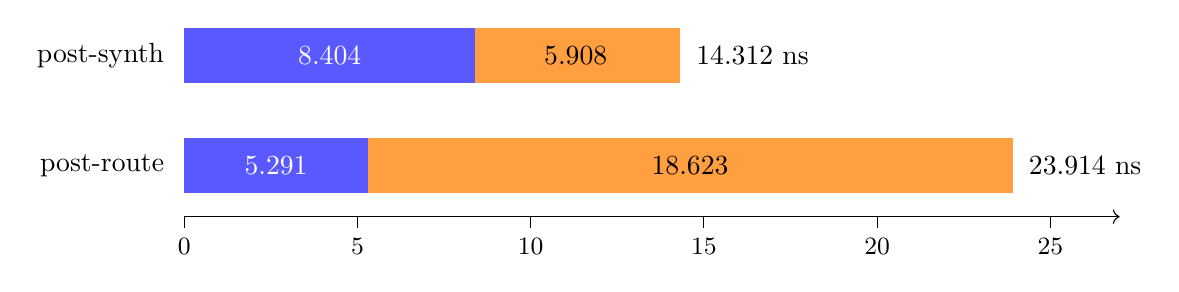
\begin{tikzpicture}[x=.44cm,y=1cm]
\fill[blue!65] (0,1.4) rectangle (8.404,2.1);\fill[orange!75] (8.404,1.4) rectangle (14.312,2.1);
\fill[blue!65] (0,0) rectangle (5.291,.7);\fill[orange!75] (5.291,0) rectangle (23.914,.7);
\node[anchor=east] at (-.3,1.75) {post-synth};\node[anchor=east] at (-.3,.35) {post-route};
\node[text=white] at (4.2,1.75) {8.404};\node at (11.3,1.75) {5.908};
\node[text=white] at (2.65,.35) {5.291};\node at (14.6,.35) {18.623};
\node[anchor=west] at (14.5,1.75) {14.312 ns};\node[anchor=west] at (24.1,.35) {23.914 ns};
\draw[->] (0,-.3)--(27,-.3);\foreach \v in {0,5,10,15,20,25}{\draw (\v,-.3)--(\v,-.45) node[below]{\small\v};}
\end{tikzpicture}\end{center}
蓝色为cell；橙色为net。post-synth为divider端点和估计互连，post-route为ID到rails端点和实际布线。真实路径route占77.875\%。不可用其倒数报告Fmax，也不能把不同端点的两行当成同一逻辑被布线恶化的精确因果实验。
\section{有限接受轨迹的15T/1T证据}
\begin{center}\begin{tikzpicture}[x=.2cm,y=.25cm]
\draw[->] (0,0)--(60,0);\draw[->] (0,0)--(0,18);
\foreach \n in {1,...,57}{\fill[blue!65] (\n,15) circle[x radius=.15cm,y radius=.12cm];\fill[orange!80] (\n,1) rectangle +(1,1);}
\foreach \n in {1,10,20,30,40,50,57}{\node[below] at (\n,-1) {\small\n};}
\node[left] at (-1,15) {15T};\node[left] at (-1,1) {1T};
\node[anchor=west] at (4,10) {蓝：context；橙：fine code};
\end{tikzpicture}\end{center}
CSV有1926沿、57接受；全部context更新后15T、fine code锁存后1T。首接受edge66/ID3：context在edge51 quiet/P0更新，fine code在edge65/P14更新。stageA为影子观察FF；未实例化真实weight/recon数据通路，未覆盖完整cfg-clear/re-enable或全序列形式证明。故不能据此直接写15/16周期例外。
\appendix

\chapter{校准原理与九模块功能详解}


审查基线为 \code{71935ab54238c7ed638f5fa66c5ffb58e10287bb}。本文件重新核对原始页图和当前源码，不把旧报告的结论当作证明。生产 RTL 未修改；只新增两个限域 bench、精确整数/Fraction 核算和两份系数镜像。该工作不是全顶层回归、模拟电路验证、新综合或 STA。


\section{先给出结论及证据边界}


\begin{itemize}
\item \textbf{静态电荷模型内，当前物理权重归约\ensuremath{\rightarrow}残差 MAC\ensuremath{\rightarrow}有符号 floor\ensuremath{\rightarrow}offset-binary 输出的代数方向一致。} 系数已经包含反馈电容/有效桥接衰减带来的级间增益，名义镜像的总信号增益为 32；重构后不能再乘/除一个 32。
\item \textbf{9 个校准模块实现片上系数装载与重构，不实现片上权重估计。} 原始论文 [00] PDF p1 右栏明确外部取得系数、片上权重修正；原文没有披露 Q30/Q32、96 位受检范围、恢复余数除法、全部学习器电路。当前工程离线估计使用独立已知输入和 SVD，这属于工程实现，不能当成原芯片学习算法的复现。
\item \textbf{PPT p18 的 lower/upper 双 dither 与论文 p1 的 RDAC dither 范围额外扩大 2 bit 尚未由当前结构核全量实现。} 当前 sampling 与 quantizer 两种模式互斥；同一个整数 dither 在量化器侧注入并从 RDAC 命令减去，或通过采样 mask 产生残差 dither，再按物理权重重构。两种模式各自可以数学闭合，但不能合并命名为原图完整双 dither。
\item \textbf{\code{cfg_ready} 只证明装载完整、基本范围与模式合法，不证明每个满幅输入都不会 \code{acc_ovf}。} 已构造合法系数镜像：把名义权重全部乘 \code{2^20}，每个系数仍 \code{<2^47}、总表和 \code{<2^60}，但 midscale 的 \code{shifted} 超出 96 位受检范围。实际 \code{cal_residue_mac} 在 6 个边界点中正确报告这些溢出。这是受保护的使用域限制，不能误报为 RTL 算术失效。
\item \textbf{发现一项必须明确的舍入语义：ties-to-even 作用于相对 \code{adc2_min_q} 的增量，不是绝对码仓中心。} 两者在奇数 min 且半整数增量时不同 1 个 Q32 LSB。RTL 与冻结合同/Python 一致，默认镜像不会碰到该角落；目前不应单独改 RTL 打破 bit-exact 合同。应统一物理数值表述与合同，或用新 ADR 同时改模型、导出、RTL 和 oracle。
\item \textbf{未新增已证实的默认配置 RTL 功能 bug。} 这不意味着全参数域、完整模拟电路、全部专利实施例或 ASIC PPA 已签核。两项新增实证（使用域与舍入）针对现有描述中需要更精确的边界。
\end{itemize}


原始输入 SHA 见 \code{input_manifest.json}；本轮数学和 bench 输入身份见 \code{calibration_evidence_manifest.json}。


\section{原文实际披露什么}


以下页码均为用户提供 PDF 的物理页号，栏号为专利纸面印刷栏号。扫描专利的 OCR 只用于检索；本次关键论断已看原始 PNG 页图。


\begingroup\small\setlength{\tabcolsep}{2pt}\renewcommand{\arraystretch}{1.25}\begin{longtable}{@{}>{\raggedright\arraybackslash}p{0.19\linewidth}>{\raggedright\arraybackslash}p{0.24\linewidth}>{\raggedright\arraybackslash}p{0.27\linewidth}>{\raggedright\arraybackslash}p{0.26\linewidth}@{}}
\toprule
\textbf{原始证据} & \textbf{页/图/条款} & \textbf{对校准链路的直接约束} & \textbf{不能据此宣称的内容}\\\midrule\endhead
[00] ISSCC 2024 正文 & PDF p1 左栏，p2 Fig. 9.8.1 & quantizer 与 RDAC 分开；8 个 slice 生成残差，8 个采样，18 个池中有 2 个备用；共用 RA；RA 示意增益 \ensuremath{\times}32 & 没有给出整数流水、系数位宽和单元逐项拟合算法\\\addlinespace[2pt]
[00] 正文 & PDF p1 右栏关于 DEM/dither 与权重修正的两段 & 两维 DEM；转移量化器结果到 RDAC 时 dither 范围扩大 2 bit；片上修正、外部产生系数 & 不能推断已知 \code{d_R=4*d_Q} 为唯一电路公式；该比例须由明确定义的单位/上下位映射及原图实施细节确认\\\addlinespace[2pt]
[00\_1] PPT & p18 lower/upper dither 框图 & dither 有进入 SADC、RDAC 输入及 RDAC 数字控制的不同路径，需分辨注入及移除位置 & 用 \code{sampling/quantizer} 两个互斥枚举模式不能构成同一时刻的完整双路径\\\addlinespace[2pt]
[00\_1] PPT & p19–20，p33–35 & gain/offset 修正；RA 采用 GMR+OTA、AZ 处理 offset/drift；ADC2 采样带宽随时间调整 & 静态 W/O 无法自动吸收时间误差、AZ 噪声代价、动态参考未稳定等效应\\\addlinespace[2pt]
[09] US10516408B2 & PDF p32 栏26 claim 1/3/9/14；p33 栏27 claim 17/19 & 采样时间常数匹配的多个 DAC 跟随数字估计；合并残差；数字操作块可修改各 slice 控制词；多个 slice 降低热噪声 & 没有规定当前 Q30/Q32、固定 16 相位或片上 SVD；数字逻辑不能证明模拟时间常数匹配\\\addlinespace[2pt]
[10] US10505561B2 & PDF p35 栏24 claim 1–12；p36 栏25–26 claim 13–24 & RDAC 采样注入与量化器注入可分开；第一/第二 dither 可有整数/小数分量；部分分量可在后级数字结果移除 & 必须逐项画注入/粗码修改/后级移除的路径，不能只验证最终数值便宣称所有 claim 均已实现\\\addlinespace[2pt]
[11] US10511316B2 & PDF p46 栏29–30 claim 1/2/7/8；p47 栏31–32 claim 15/17/20 & \code{shared/additional} 部分在合作 DAC 之间分配；main/sub bridging；已知注入可用于 \code{dither/calibration}；动态选 K/L slice；二维索引 & 仅打乱粗码逻辑位置不能代替物理单元的选择记录；没有规定完整系数训练电路\\\addlinespace[2pt]
\bottomrule\end{longtable}\endgroup


原始页图：\code{reference_pages/00_p1.png}、\code{00_p2.png}、\code{00_1_p18.png}、\code{09_p32.png}、\code{10_p35.png}、\code{10_p36.png}、\code{11_p46.png}。对应 OCR 为 \code{reference_text/*_p*.ocr.txt}。纸面 claim 与工程覆盖的对照是技术范围审查，不构成法律意见。


\subsection{对 dither 覆盖的精确判断}


当前 \code{sar_structural_ctrl.sv:199–202} 输出量化器 dither；\code{:214–218} 只有 \code{quantizer_en=1} 才从粗码反号减去 \code{current_dither}。采样轨由 \code{:204–206} 与 \code{unit_therm} 产生，实际采样 mask 的四列物理权重参与校正。\code{calib_regs.sv:116–118} 拒绝 sampling 和 quantizer 同时开启。


因此：量化器模式与 [10] claim 13 的一般方法具有部分对应；采样 dither 经残差后在后级重构移除，与 claim 21/23 的一般路径具有部分对应。但 sampling 模式没有根据该 sampling dither 同时改变粗码的现行控制，第二分量的小数位及后级移除也没有独立接口。不能把这种部分对应升级成 claim 1–12 或 PPT p18 全部拓扑复现。


精确有效的设计动作是先定义 \code{d_Q}、\code{d_R}、低/高分量、每个分量的物理单位和符号，再列四个边界：SADC 输入、RDAC 采样输入、RDAC 数字命令、ADC2 数字重构。只要该分量已经通过实际 RDAC 开关命令计入 \code{rails}，就不能再无条件加入公共 \code{I} 做第二次扣除。当前量化器模式应让公共 \code{inj_q} 不再包含已移除的量化器 dither。


\section{从电荷守恒重新推导重构式}


\subsection{物理残差，不从数字粗码直接猜电压}


对固定物理 slice 的一个有效单位，定义正权重 \code{w_j=C_j,eff/C_F}。main 单元 \code{C_j,eff=C_j}，sub 单元的权重含桥接衰减 \code{beta}。这是 RA 处在理想虚地/静态稳定边界内的有效系数；其值可以经过片外标定，不能从原文图直接读出全部实物数值。


令 normalized 输入 \code{x=V_in/V_fs}、已知公共注入 \code{i=V_inj/V_fs}、\code{on_j=1} 表示转换底板接正参考。转换底板 normalized 电压为 \code{2*on_j-1}。普通信号单位在采样时接 \code{x+i}，因此该单位的残差贡献为


\code{w_j * [x+i-(2*on_j-1)] = w_j*x + w_j*i + w_j*(1-2*on_j)}。


若单位用于 sampling dither，它不接信号，采样底板为 \code{r_j+i}，其中 \texttt{r\_jin\{-1,+1\}}。此时贡献为


\code{w_j * [r_j+i-(2*on_j-1)] = w_j*i + w_j*(1-2*on_j+r_j)}。


合并以后得到


\code{F_phys = O + G*x + T*i + R}，


\code{T = sumw_j}，\code{G = suma_j*w_j}，\code{R = sumw_j*s_j}，


其中普通单位 \code{a=1,s=1-2*on}；sampling dither 单位 \code{a=0,s=1-2*on+r}。由 \code{r} 与转换底板轨相减，sampling 单位的 \code{s} 是 \code{-2/0/+2}，不是只取 \ensuremath{\pm}1。


因而


\code{x = (F_phys-O-R-T*i)/G}，条件是 \textbf{G>0 且测得的 F 属于同一物理开关/epoch/样本}。


这解释了为什么必须记录 DEM 之后的物理 ID 与开关 mask，而不能只保存粗码。不同 active slice 的失配权重总和不同；\code{T/G} 可以随选择改变；不应把全部转换的 gain 固化成 32，也不能用下一组 slice 的系数解释上一组残差。


\subsection{桥接消元为什么可用逐单位有效权重}


在 main 顶板 P 近似虚地、sub 顶板 Q 浮置的理想边界，令 sub 电容和为 B，桥接电容 C\_C，sub 寄生为 C\_p：


\code{(C_C+B+C_p)*V_Q = sum_sub C_j*(V_convert,j-V_sample,j)}；


\code{C_F*V_R = sum_main C_j*(V_sample,j-V_convert,j) - C_C*V_Q}。


消去 Q 后，sub 项变为 \code{beta*C_j}，其中 \code{beta=C_C/(C_C+B+C_p)}。所以静态 \code{w_j=beta*C_j/C_F} 能同时承担 main/sub 比例与 RA 增益。该结论是对明确边界的电荷推导，不是对动态真实 GMR/OTA、漏电、参考瞬态或开关寄生注入的全电路证明。


当前 \code{src/adi_model/weight_calibration.py:1–12} 的线性模型与 \code{:176–201} 的逐单元 terms 和此推导一致：\code{b_minus_dac} 包含公共注入与采样轨减去实际 DAC 轨；\code{signal} 对 sampling mask 置 0。该模型依赖静态条件；它不能拟合掉所有频率相关误差。


\subsection{定点化与最终码}


权重整数 \code{W=round(w*2^30)}；电压整数 \code{F/O/I} 以 Q32 承载；\code{R=sumW*s}、\code{T=sumW}、\code{G=sumW*a} 都仍以 Q30 承载无量纲量。于是


\code{num=(F-O)*2^30 - R*2^32 - T*I}，


\code{x_hat=num/(G*2^32)}，


\code{word=floor((x_hat+1)*2^19)}，


等价于


\code{shifted=(num+G*2^32)*2^20}，


\code{word=floor(shifted/(G*2^33))}。


因为 G 为正，整数嵌套 floor 恒等式允许 \code{A1=floor(shifted/2^33)}，然后 \code{word=floor(A1/G)}，\textbf{对负 shifted 也成立}。不能用向零截断代替 floor；输出需要先与有符号 0 和 \code{2^20} 比较，最后饱和到 20 位。


当前镜像 \code{sim/vectors/registers_paper_literal.json}：main W=\code{67108864=2^26}，sub W=\code{8388608=2^23}，8 个 active slice 的名义 G=\code{34359738368=32*2^30}。因此 \code{G/2^30=32} 已经承载论文 Fig.9.8.1 的 \ensuremath{\times}32。它不是要在数字结果之后再乘 32 的信号放大器。


\subsection{系数学习与在线重构必须分开评价}


本工程学习器的设计矩阵来自已知输入和数字记录：对每个样本，每个物理系数的 feature 为 \code{a*x_known + b-V_DAC}，再加 offset 常数列。默认有 \code{18*71+1=1279} 个未知量；至少要求 \textbf{样本数>1279、矩阵满列秩、合理的条件数与独立 holdout}。重复采集同一个不可辨识状态不会自动增加秩。


\code{src/adi_model/weight_calibration.py:299–381} 执行 rank-revealing SVD、检查有限性/秩/正权重，再冻结系数；RTL 不含这些操作。SVD 仿真训练的受控已知输入精度、参考不确定度、码量化偏差和噪声条件也不是原芯片在线校准电路的证明。应保留训练/验证不同数据、不同激励、已知输入来源及温度漂移信息，不用待校准 DUT 的真实电容、输入真值或理想残差当作硬件可读量。


\section{逐模块功能、状态及推导电路}


以下行号是当前基线源码的精确行号。寄存器 bit 数为代码可推导数量，不是新的综合实测资源；综合会常量传播、删冗余或重映射。


\subsection*{\code{weight_store.sv:32–149}}
\noindent\textbf{接收/输出与本质功能}：保存 18\ensuremath{\times}71 物理 W；给出全表、行总和、选中写地址读回和完整性\par
\noindent\textbf{状态、时序、错误资格}：\code{:95–111} 拒绝非法地址/0/\ensuremath{\ge}2\textasciicircum{}47/活动配置写入；\code{:113–126} 用本行旧值更新缓存；\code{:130–145} reset 清数值，clear 只清 written，换 epoch 重写所有项\par
\noindent\textbf{可推导电路及主要风险}：1278\ensuremath{\times}47=60,066 个非恒零系数 bit；written 1,278 bit；18\ensuremath{\times}54=972 行和 bit，合计 \textbf{62,316 FF 候选}。18 路 71:1 old-word mux、行更新减加及配置读回。全表并行输出导致 FF/宽连线，不能直接替换成单口 RAM\par
\subsection*{\code{calib_regs.sv:52–160}}
\noindent\textbf{接收/输出与本质功能}：三个 Q32 标量+四控制位；validate 提交配置\par
\noindent\textbf{状态、时序、错误资格}：\code{:109–128} clear 优先；忙/写冲突拒绝提交；\code{sampling+quantizer} 互斥，min<max，权重/标量完整。活动 epoch 禁止改值\par
\noindent\textbf{可推导电路及主要风险}：192 标量+3 完成+4 控制+ready+32 错误\ensuremath{\approx}\textbf{232 bit}，少量比较器/资格 mux。\code{P_ADC2_BITS} 不消费，不能当成完成任意 ADC 后端适配\par
\subsection*{\code{cal_sample_context.sv:32–69}}
\noindent\textbf{接收/输出与本质功能}：current\ensuremath{\rightarrow}residue\ensuremath{\rightarrow}fine，保存物理 ID、main/sub mask、采样轨、注入\par
\noindent\textbf{状态、时序、错误资格}：phase9 保存当前残差包；下周期 quiet/phase0 把旧 residue 交给 ADC2。reset/disable 丢两包。两 strobe 同沿时 fine 收旧 residue，未实现 capture bypass；生产相位将其分开\par
\noindent\textbf{可推导电路及主要风险}：CW=709，两份完整 payload+4 valid/bad=\textbf{1,422 bit}；本模块不保存模拟电压，也不按系数 epoch编号，只依赖配置锁定/取消\par
\subsection*{\code{cal_weight_reduce.sv:51–185}}
\noindent\textbf{接收/输出与本质功能}：实际物理选中行与 on mask\ensuremath{\rightarrow}T/G/R\par
\noindent\textbf{状态、时序、错误资格}：\code{:73–85} 维度检查+重复/越界 ID异常；重复ID按物理行OR只计一次并标 invalid。\code{:67–71} G=T\ensuremath{-}mask，\code{:185} rails=total\ensuremath{-}2*on+dither\par
\noindent\textbf{可推导电路及主要风险}：无 FF。18\ensuremath{\times}8=144 个 5bit equality 选行；28 个 ID 重复比较；on 1278 非零候选叶、1277 潜在有效加法节点，深度约11；生产行和缓存树18叶/17节点；4列\ensuremath{\times}18叶/68节点，再mask/rail各3节点。宽叶输入/扇出/拥塞比“for循环长度”更能预示布局风险\par
\subsection*{\code{adc2_dec.sv:57–104}}
\noindent\textbf{接收/输出与本质功能}：raw ADC2 integer\ensuremath{\rightarrow}Q32 相对量程的码仓增量再加min\par
\noindent\textbf{状态、时序、错误资格}：组合。\code{:81–87} 形成 \code{(2c+1)*(max-min)}；\code{:91–95} 相对增量RTE；\code{:98–104} 宽加、溢出钳位。载入器检查min<max\par
\noindent\textbf{可推导电路及主要风险}：有效 \textbf{13\ensuremath{\times}65} 可变量程乘法（不是按decl名义78\ensuremath{\times}78）；固定右移是连线，RTE低位比较+增一；min加法。合法升序端点下 fine 始终在min/max之内，numeric ovf不可达，不能从raw code判断模拟ADC2 over\par
\subsection*{\code{cal_residue_mac.sv:33–88}}
\noindent\textbf{接收/输出与本质功能}：同一 sample快照\ensuremath{\rightarrow}num\ensuremath{\rightarrow}offset-binary偏置\ensuremath{\rightarrow}A1\par
\noindent\textbf{状态、时序、错误资格}：组合，\code{op1/op2/op3/num/den/shifted}受检范围[-2\textasciicircum{}95,2\textasciicircum{}95)。any\_ovf时 A1无有效数值保证，不能使用其看似合理的截断值\par
\noindent\textbf{可推导电路及主要风险}：宽差/移位/加减/比较器；唯一可变量乘是 \textbf{unsigned total \ensuremath{\times} signed injection}，源码64\ensuremath{\times}64语义范围，经综合可能缩窄，不能把132bit sign extension计成132\ensuremath{\times}132乘法。该级的乘法+宽减法+异常检查要独立看STA\par
\subsection*{\code{div_floor.sv:50–163}}
\noindent\textbf{接收/输出与本质功能}：\code{q=floor(A1/G)}\par
\noindent\textbf{状态、时序、错误资格}：只idle/start接受。P5用13次迭代，P7用9次；busy start忽略。zero denominator定长结束q0/err1；宽分母不截断；负非整除补\ensuremath{-}1；同步reset取消\par
\noindent\textbf{可推导电路及主要风险}：P5每拍\textbf{5个63bit恢复减法/借位\ensuremath{\rightarrow}选择}串联；P7串7个。除法器寄存器约P5 329bit/P7 325bit，不是展开全部63级的单拍除法。组合级数与busy周期折中，不应只减P\_STAGES却忽略16相位容量\par
\subsection*{\code{recon_core.sv:81–279}}
\noindent\textbf{接收/输出与本质功能}：归约/ADC2\ensuremath{\rightarrow}stageA\ensuremath{\rightarrow}MAC/div\ensuremath{\rightarrow}提交\par
\noindent\textbf{状态、时序、错误资格}：\code{:250–260} 只有ready/start/!busy采样；\code{:261–267} 下沿采样本样本MAC异常并launch；\code{:183–203} divider/busy；COMMIT时busy0，可接受下一start，旧ID由NBA保留；ready下降取消。接受\ensuremath{\rightarrow}valid=P5 15/P7 11完整间隔\par
\noindent\textbf{可推导电路及主要风险}：stageA 418 payload+5状态\ensuremath{\approx}\textbf{423bit}，算术在子模块。系数无需每次拷贝，只要完整epoch冻结。改流水必须同步ID/flags/context，否则数值可对而样本关系错误\par
\subsection*{\code{cal_output_stage.sv:34–78}}
\noindent\textbf{接收/输出与本质功能}：candidate\ensuremath{\rightarrow}dout/ID/current flags，保持三个sticky\par
\noindent\textbf{状态、时序、错误资格}：complete \&\&ready发valid。acc/gain错误仍发完成，但保留最后合法dout/clip；ADC2 numeric ovf单独报告不阻止字更新。clear与新错误同沿新错误优先；ready0丢提交\par
\noindent\textbf{可推导电路及主要风险}：\code{OUT20+ID32+flags5+valid1+clip2+sticky3}\ensuremath{\approx}\textbf{63bit}。\code{dout_valid} 表示完成事件，必须联合当前flags；不能拿sticky历史位当当前结果资格\par


\subsection{row\_total 缓存是不是偷偷改变了校准}


没有。\code{weight_store} 仅替换写入所在行的旧值，再加新值，clear epoch时保留数值/行缓存并清完成 bitmap。新 epoch 第一次重写必须减去保留的旧 W。当前 \code{:118–121} 就做这个操作，未把“本epoch没写过”误认为旧值为零。


生产 \code{recon_core} 启用 \code{P_USE_ROW_TOTALS=1}（顶层 \code{sar20_digital_core.sv:628–637}），仅将总和 T 的归约改为18行缓存树；on-tree和dither列仍取物理W。\code{cal_weight_reduce.sv:111–112} 明确调用方承担 \code{row_total[s]==sumw_rom[s,u]}。\textbf{独立模块用户若打开该参数却提供陈旧缓存，会静默得到错误T/G/R；顶层使用同一weight\_store输出保证其一致。} 这是接口前置条件，不是顶层已证实 bug。


\subsection{为什么当前存储不能自然变 BRAM/SRAM}


配置写入是单地址，重构读出却是物理全表并行接口：568个活跃项、动态on选择，还需dither列权重。即便每帧16拍，按568项全读也平均需35.5项/拍；如果重构归约能用的窗口更短，带宽更高。RAM方案必须给出银行数、每bank读端口、地址冲突、所需位宽和周期，并在保持采样/重构ID的条件下完成。


另一个候选是围绕当前二维DEM的前缀/分组和缓存，但它需证明所有main/sub bridging、二位旋转、slice集合与sampling mask的等价关系，不能用一维63环前缀替换当前8\ensuremath{\times}8跳过占位单元的二维映射。


\section{数值边界与新增最小实证}


\subsection{位宽、符号、floor及溢出核对}


\begin{itemize}
\item W只允许 \code{0<W<2^47}，读入时按无符号零扩展；positive“signed Q30”与“无符号 bit型存储”的表述并不冲突，高bit为0。电压、rails、有符号分子必须符号扩展，不能把负电压或负word改成unsigned。
\item \code{cal_residue_mac.sv:57–66} 的 \code{F-O} 保留65bit，乘积total\ensuremath{\times}inj先对total零扩展再signed乘；其132bit临时量用来形成和检查精确受检操作数，随后才合法裁位。
\item \code{:76–87} 的97bit s1可容纳两个已受检量之和，117bit shifted容纳完整乘\code{2^20}；top22bit检查等价于signed shifted装入96位。若任何前置op非法，A1允许成为截断位型，但any\_ovf禁止合法字更新。
\item den=\code{G*2^33}的受检上界对应 \code{G<2^62}；这不是shifted的更严格工作范围，不能把该上界当成全链路无溢出保证。
\item \code{div_floor} 的最小负数用unsigned幅度可保存；大于numerator域的64bit分母保留highbit意义。组内qbit MSB顺序正确，负非整除用非零remainder下修。valid denominator为正时不需signed除数。
\item signed剪裁在 \code{recon_core.sv:201–206} 先于截取20位；低/高剪裁与acc溢出、gain结构错误和模拟饱和不是同一件事。
\end{itemize}


\subsection{完整载入不等于满幅均可工作：6点MAC实证}


当 \code{num=0}（输入等效midscale），\code{shifted=G*2^52}，故96位上界要求 \textbf{G<2\textasciicircum{}43}。对恰好\code{x=+1}，\code{shifted=G*2^53}，要求 \textbf{G<2\textasciicircum{}42}。如果把严格输入域写成\code{x<+1}，\code{G=2^42}可在该开区间内通过，但端点或量化后的候选值仍需实际检查；不能笼统给出满幅都安全。


两份镜像沿用原后端量程，offset设为该镜像raw ADC2 code341的精确解码值26215。slice IDs=0..7，每行main物理0..31接正参考、sub全负、sampling关、I=0，则R=0且F\ensuremath{-}O=0。


\subsection*{\code{calibration_domain_nominal_mirror.json}}
\noindent\textbf{最大W}：67,108,864\par
\noindent\textbf{全表和}：77,309,411,328\par
\noindent\textbf{本样本G}：34,359,738,368\par
\noindent\textbf{\code{shifted}}：\code{2^87}\par
\noindent\textbf{资格}：装载谓词合法，MAC合法\par
\subsection*{\code{calibration_domain_scaled_2pow20_mirror.json}}
\noindent\textbf{最大W}：\code{70,368,744,177,664}\par
\noindent\textbf{全表和}：\code{81,064,793,292,668,928}\par
\noindent\textbf{本样本G}：\code{36,028,797,018,963,968}\par
\noindent\textbf{\code{shifted}}：\code{2^107}\par
\noindent\textbf{资格}：装载谓词仍合法，MAC acc\_ovf\par


实际 \code{cal_residue_mac} bench还测试midscale的 \code{2^43-1/2^43} 与正满幅的 \code{2^42-1/2^42} 两对边界；6/6如推导。日志为 \code{calibration_domain_run.log}，终止标记为 \code{CALIBRATION_DOMAIN_PASS cases=6 scope=MAC_ONLY_NOT_FULL_TOP}。不使用非法A1作为通过证据。


该bench没有运行全表加载、全顶层或模拟回路，镜像“装载合法”由精确的单系数/总和谓词核算，不应改写成已经在顶层载入并物理运行成功。建议软件导出器同时报告：每种slice集合/采样模式的G极值、原始ADC量程/offset/I边界、6个受检op的最大值与margin。要把更多拒绝搬到validate，先证明拒绝条件不会错误排除允许使用的局部量程，并记录为新的合同。


\subsection{ties-to-even 的作用点：9点ADC2实证}


工程合同和RTL定义为


\code{C = min_q + RTE(((2c+1)*(max_q-min_q))/2^(N+1))}。


如果“把绝对码仓中心按Q32最近偶数取整”的物理文字定义是目标，则应比较


\code{P = RTE(min_q + ((2c+1)*(max_q-min_q))/2^(N+1))}。


RTE不满足任意整数平移不变性；min为奇数时，恰好半整数会改变偶数判断。


\begingroup\small\setlength{\tabcolsep}{2pt}\renewcommand{\arraystretch}{1.25}\begin{longtable}{@{}>{\raggedright\arraybackslash}p{0.19\linewidth}>{\raggedright\arraybackslash}p{0.24\linewidth}>{\raggedright\arraybackslash}p{0.27\linewidth}>{\raggedright\arraybackslash}p{0.26\linewidth}@{}}
\toprule
\textbf{min/max/code} & \textbf{精确中心（Q32整数单位）} & \textbf{当前C} & \textbf{绝对中心P}\\\midrule\endhead
1 / 4097 / 0 & 1.5 & 1 & 2\\\addlinespace[2pt]
1 / 4097 / 1 & 2.5 & 3 & 2\\\addlinespace[2pt]
1 / 4097 / 4094 & 4095.5 & 4095 & 4096\\\addlinespace[2pt]
\ensuremath{-}4097 / \ensuremath{-}1 / 0 & \ensuremath{-}4096.5 & \ensuremath{-}4097 & \ensuremath{-}4096\\\addlinespace[2pt]
0 / 4096 / 0 & 0.5 & 0 & 0\\\addlinespace[2pt]
原镜像 / code341 & \code{107374865/4096 = 26214.566650390625} & 26215 & 26215\\\addlinespace[2pt]
\bottomrule\end{longtable}\endgroup


最后一行用精确有理值计算。当前镜像delta=\code{644245094}，二进制因子仅2，不能让奇数 \code{(2c+1)} 的乘积在除8192时落于半整数，因此这一舍入角落不影响当前默认镜像。


\code{adc2_rounding_semantics_tb.sv} 直接实例化当前ADC2：9案例，6个C/P差异，全部RTL严格符合C。日志为 \code{adc2_rounding_semantics_run.log}，标记 \code{ADC2_ROUNDING_SEMANTICS_REPRODUCED cases=9 differences=6}。这是\textbf{合同和文字物理定义待统一}，不是新发现的默认RTL偏离oracle。


在Gphys=32时1 Q32 LSB相当于未量化输出 \code{2^-18 LSB20}，很小；但当最终floor阈值恰好夹在两个数之间，仍可能表现为1code差，不能断言“永远不影响最终码”。若选择绝对中心RTE，应把increment的tie parity改为\code{(q_shift+min_ext)[0]}等价语义，并同步修改全部模型/导出/回归，而不是单改RTL。


\subsection{有限独立计算与参数边界}


\code{calibration_math_check.py} 的精确Fraction/整数结果：


\begin{itemize}
\item 6组端点\ensuremath{\times}4096码=\textbf{24,576} ADC2计算，当前增量RTE与显式合同全匹配；相对绝对中心RTE差8192例，全为1Q32 LSB。
\item \textbf{5,000} 随机signed大整数，直接有理floor与剥去\code{2^33}的嵌套floor完全一致。
\item 小宽度 WA=2..6、WD=1..8、group=1/3/7，共 \textbf{186,744} 计算，含最小负数、比numerator宽的分母、padding及非整除，恢复余数算法与整数floor全一致。该项是独立算法计算，不是任意参数RTL形式证明。
\item 两份1278系数镜像的单权重合法域、全表和、实际T/G/R、ADC2code341、MAC资格均由精确整数封存。
\end{itemize}


几何参数与header常量不能混淆：weight\_store维度只支持\code{slice1..32/unit1..128}；ID5bit、unit7bit固定。reduce约束\code{SUM_BITS>=W_BITS+ceil(log2(N_TERMS))}，要求P\_DIT\_N\ensuremath{\ge}1与有效DIT\_BEG；若sampling打开而DIT\_END超过实际单元则invalid。recon/cal\_mac的格式来自冻结header，不是完整通用宽度算术库；改W\_BITS/ACC/V/OUT需重生params并重新证明所有拓扑和常量，当前weight\_store的47/48/60以及ROW\_BITS有意绑定冻结格式。


\subsection{Q30 系数的条件误差界及缩位代价}


该界只评价\textbf{对同一组已确定有效物理系数的定点量化}，不评价训练误差、真实噪声、参考误差或增益漂移。设 \code{hat(w)=w+delta}，每项 \code{|delta|<=2^(-F_W-1)}，I=0、输入x\ensuremath{\in}[-1,1]，普通项\code{s=+/-1}、sampling项\texttt{a=0,sin\{-2,0,+2\}}，因此 \code{|a*x+s|<=2}。使用精确物理F而改用量化系数重构时


\code{hat(x)-x = -sumdelta*(a*x+s)/hat(G)}。


若另外能证明 \code{hat(G)>=32}、最多N=568项，则20bit未floor输出的误差上界为


\code{E_code <= 2^19 * 568 * 2 * 2^(-F_W-1) / 32}。


\begingroup\small\setlength{\tabcolsep}{2pt}\renewcommand{\arraystretch}{1.25}\begin{longtable}{@{}>{\raggedright\arraybackslash}p{0.25\linewidth}>{\raggedright\arraybackslash}p{0.32\linewidth}>{\raggedright\arraybackslash}p{0.39\linewidth}@{}}
\toprule
\textbf{权重小数位 F\_W} & \textbf{单项量化误差界} & \textbf{条件下的输出误差界（LSB20）}\\\midrule\endhead
30 & \code{2^-31} & \textbf{0.0086669921875}\\\addlinespace[2pt]
26 & \code{2^-27} & \textbf{0.138671875}\\\addlinespace[2pt]
22 & \code{2^-23} & \textbf{2.21875}\\\addlinespace[2pt]
\bottomrule\end{longtable}\endgroup


这说明Q30在上述工作域内有充分量化余量，Q22不能在同一最坏界下支持小于1LSB的数字权重量化预算。不能把三行作为不带前提的所有配置保证：\code{cfg_ready}不保证hat(G)\ensuremath{\ge}32，也不限制真实输入/I边界；名义sampling四列mask把G从32降为31.75，因此采样模式须用实际G\_min重算（Q30界约0.00873524LSB，而不是直接引用0.00866699）。如果I不为0，应把分子界换为\code{2+|I|}；如果hat(G)趋近0，误差会被任意放大。


这些是\textbf{未floor码值}的误差界。只要输入候选恰好靠近整数阈值，0.0087LSB的连续差也可能导致最终floor输出相差1code；不应把小于1LSB的连续界误写成bit-exact全码一致。ADC2量化、offset/RTE和外部标定误差预算需另行相加或按照其统计关系评价。


\section{结果资格及模型覆盖仍需注意}


\code{dout_valid} 是完成通知，不自动等于“本样本有效测量”。acc/gain错误时word沿用前一合法样本，当前ID/flags仍更新。上位机必须保留ID与flags，否则一笔无效转换会看起来像前一笔数据重复。历史sticky也不能代替当前flags。


模拟 \code{adc2_over/rdac_ovf/ra_sat} 与 \code{adc2_dec} 的numeric ovf不同。当前顶层 \code{sar20_digital_core.sv:680–706} 把模拟故障与被捕获context关联后进入sticky状态，但五位 \code{dout_flags} 不含单独的本样本模拟故障位。若未来要逐样本评分、discard、闭环训练或设备在线故障诊断，应增加明确的同ID模拟质量metadata，或规定能无歧义恢复其关联的事件接口。当前sticky说明“发生过”，不够说明“具体哪笔数字输出可用于标定”。这是接口/验收建议，本次未将它标为新的已证实默认RTL bug。


静态校正无法替代输入settling、参考settling、时钟skew、泄漏/记忆、瞬时开关注入、非线性RA以及AZ/ADC2带宽噪声的验证。原文[00] p1、PPT32–35已指出这些误差；W/O恒定拟合把它们“吸收掉”只在特定训练信号条件下偶然成立，并不能支持全频率/温度/输入幅度结论。


\section{综合风险优先级与可评估改进}


\subsection{已可推导的主要成本}


权重FF候选62,316；上下文约1,422；配置约232；重构stageA约423；除法器约325/329；输出约63。重量级成本是系数保存和物理归约，不是有限状态机的状态bit。on归约物理树按1278项布线，生产总和采用18行缓存，但on-tree仍约11层组合加法；物理active/mask分发、权重叶子扇出、adder placement和rail最后加减都可能构成长互连。


这些估算不包含RTL顶层其他模块，也不能直接换算为ASIC面积或功耗。\code{wire [63:0]}加法的声明不等于每个节点都真的需要64bit全加器，零扩展/固定padding可使部分节点缩窄；反过来，系统数学上的“最多8行活跃”不一定被综合器从二进制decode推导为每条进位的范围约束。应查mapped cell/netlist而不是用数学上限冒充映射资源。


\subsection{建议顺序}


\begin{itemize}
\item \textbf{先收紧语义说明}：写明片外训练/片上重构、增量RTE、真实有效W包含级间增益、cfg\_ready的含义、\code{sampling/quantizer/}双dither区别、同ID质量标志。
\item \textbf{导出侧建立范围证据}：对实际校准系数、合法slice集合、sampling mask和I边界，报告minG/maxG及6个op的range margin；小G需同时检查Q30系数误差放大，不能只验G>0。
\item \textbf{用既有真实STA定位数字结构}：先检查 ID\ensuremath{\rightarrow}\code{active/physical_on}\ensuremath{\rightarrow}\code{on_tree/row_tree/column}\ensuremath{\rightarrow}rails\_s 路径及fanout；把物理行相邻放置、局部归约、mux/adder结构作为单变量实验。新增pipeline需把ID、F、O、I、G、T、R与异常全对齐，并重新验证P5/P7的16拍预算。
\item \textbf{优先评估存储带宽}：FF全表方案简单且可读，但成本很大。banked SRAM/BRAM、系数压缩/差值、精确前缀缓存必须分别给出误差证明和端口/帧预算；禁止靠删高位、减弱overflow或近似除法获得看似低面积。
\item \textbf{优化divider不能只改展开数}：P5/P6/P7要相同输入/时钟/约束对比，记录局部critical path、busy周期、重构接受间距、全顶层开关与flags对齐；P6需要覆盖当前runner未默认注册的中间选择。
\item \textbf{双dither应作为明确的新功能里程碑}：先用原始图把各分量单位/注入节点/数字移除边界写成契约，独立电荷求解器与holdout给出闭合，再扩RTL上下文/接口和拟合激励。当前已有单路径计算结果不构成这个里程碑的证据。
\end{itemize}


本轮结论足以把目前工程的校准数学、功能与潜在综合电路解释清楚；它不把原文未披露的细节填成事实，也不以CI成功代替物理实现验收。
\chapter{控制、采样与专利原理详解}


审查对象为 \code{71935ab54238c7ed638f5fa66c5ffb58e10287bb} 的当前 RTL。原文身份以本目录 \code{input_manifest.json} 为准。本文直接查看 [00] PDF p1/p2、[00\_1] slides12/19/24–26/30/31/34/35，以及 [09] Fig9/10、[10] claims、[11] claims、[12] Fig8 与正文/claims、[13] Fig2/6/11/12 与 claims、[14] Fig2/8–11 与 claims 原始页面。OCR 仅作检索，图是原文依据。当前生产源码未改动；新增有限见证是外部审查附件，不能冒充新综合、STA、模拟或形式等价证据。


\section{判断必须分四层}


\begin{itemize}
\item \textbf{原文明示的架构}：两套 coarse quantizer、共享 Flash、独立 RDAC、18 个 residue slices 中 8 个采集/8 个转换/2 个备用；coarse 为 9-bit；RDAC跟随已决 SAR 码；共享 RA/ADC2；相同 TP 关键下降沿及本地 EN/hold-low 支路；粗参考预充电\ensuremath{\rightarrow}准确外部参考；dither 范围增强 2 bit；slice 与 \code{horizontal/vertical} DEM。
\item \textbf{当前工程实现}：3-bit Flash种子+6次同步二进制SAR决策、12-bit同步 ADC2、16-clock帧、63+8单位展开、LFSR及确定性状态序列、扫描式8/18选择、\ensuremath{\pm}1零和bridge、Q格式/配置epoch/数字回读。9-bit coarse本身不是工程猜测；具体基数、逐拍控制和ADC2=12-bit是工程选择。PPT“>12b AC matching”是 SADC 与 RDAC 匹配，不能据此认定 ADC2 是12-bit。
\item \textbf{已有但限定范围的诊断契约}：模拟bad以独立sticky保存；每结果5-bit flags只记录数字算术与clip；宏比较器valid/data必须同步；模拟错误读回须保持到quiet观察沿。上述契约不是完整模拟错误逐样本账本。
\item \textbf{尚未完整覆盖或模拟宏承担}：论文dither两端不同范围、专利tracking预设、动态 ADC2采样带宽、晶体管级AUX/参考/RA/非交叠/level-shift/共享关键沿的物理实现。专利引用不能证明论文实际采用每个可选实施例。
\end{itemize}


\section{当前逐沿数据流程与真实预算}


所有 phase 指上升沿前的旧相位；NBA 后安装下一相位。\code{sar_structural_ctrl.sv:281} 的 \code{recon_start} 是组合 wire，而不是 phase15 分支中注册的 NBA 信号。\code{recon_core.sv:250–260} 在该 pre-phase15 沿直接接受 Stage A；下一 pre-phase0 沿才替换 fine context。因此不能把结果接受挪到下一phase0，或把整帧16拍无条件设为所有路径的 multicycle。


\begingroup\small\setlength{\tabcolsep}{2pt}\renewcommand{\arraystretch}{1.25}\begin{longtable}{@{}>{\raggedright\arraybackslash}p{0.19\linewidth}>{\raggedright\arraybackslash}p{0.24\linewidth}>{\raggedright\arraybackslash}p{0.27\linewidth}>{\raggedright\arraybackslash}p{0.26\linewidth}@{}}
\toprule
\textbf{旧phase沿} & \textbf{该沿的数字行为} & \textbf{NBA后状态/归属} & \textbf{审核位置}\\\midrule\endhead
15\ensuremath{\rightarrow}0 & TP寄存器拉低；上一笔fine context由当沿Stage A接受（如launch=1） & phase0 quiet窗口，fine context仍旧 & analog\_phase:42–47；structural:281；recon:250\\\addlinespace[2pt]
0\ensuremath{\rightarrow}1 & quiet\_sample冻结当前acquiring dither/injection；旧residue packet转为fine packet；coarse bank翻转 & 新fine context、fine/acq读回bad已冻结；两个SAR尚未start & structural:315–320；context:64–68\\\addlinespace[2pt]
1\ensuremath{\rightarrow}2 & 旧acquiring slices晋升converting；从补集选下一acquiring组；sharedFlash种子启动选中coarse；上笔context启动fine & coarse busy、trial MSB待比较；fine busy；acquisition EN更新；DEM/dither取旧输出后推进 & pool:66–81；structural:122–165/322–328\\\addlinespace[2pt]
2\ensuremath{\rightarrow}3 & coarse第1次决定；RDAC此沿先装上一沿start产生的已决seed & resolved更新，本次accepted bit待下一沿装RDAC & trial:54–75；structural:236–250\\\addlinespace[2pt]
3–7 & coarse继续低6bit逐次比较；fine继续12bit比较 & 旧resolved\_valid驱动RDAC，trial不直接驱动RDAC & 同上\\\addlinespace[2pt]
7\ensuremath{\rightarrow}8 & coarse最后一次有效比较可使done NBA变1；registered coarse cancel NBA变1 & coarse compare enable关闭，最后resolved已就绪 & structural:312；trial:69–75\\\addlinespace[2pt]
8\ensuremath{\rightarrow}9 & 读取旧coarse\_done；装最终resolved至RDAC；coarse SAR同步取消 & coarse\_ok冻结；ref\_precharge关闭，准确reference尚未打开 & \code{structural:238/330}–332；phase:44–47\\\addlinespace[2pt]
9\ensuremath{\rightarrow}10 & 冻结当前RDAC物理ID/掩码/轨/injection及rdac\_over；准确参考/RA开始 & residue packet属当前样本，fine packet仍前一笔 & context:53–57；phase:45–47\\\addlinespace[2pt]
13\ensuremath{\rightarrow}14 & fine最后一次有效比较可done；fine acquisition注册打开 & fine\_done NBA变1，fine cancel NBA变1 & \code{structural:307/313}；trial:69–75\\\addlinespace[2pt]
14\ensuremath{\rightarrow}15 & 读取旧\code{fine_done/fine_resolved}并锁存fine\_code & fine\_ok/code稳定；细SAR取消；phase15组合launch可为1 & structural:334–337\\\addlinespace[2pt]
下一15\ensuremath{\rightarrow}0 & Stage A接受冻结fine packet及fine\_code & context不会在此沿被换成下一笔 & structural:281；context:64；recon:250\\\addlinespace[2pt]
\bottomrule\end{longtable}\endgroup


在期望 ASIC640MHz 时钟预算 \code{T=1.5625ns} 下，以下只是\textbf{源码逐沿换算}，不是时序或模拟实测：


\begingroup\small\setlength{\tabcolsep}{2pt}\renewcommand{\arraystretch}{1.25}\begin{longtable}{@{}>{\raggedright\arraybackslash}p{0.19\linewidth}>{\raggedright\arraybackslash}p{0.24\linewidth}>{\raggedright\arraybackslash}p{0.27\linewidth}>{\raggedright\arraybackslash}p{0.26\linewidth}@{}}
\toprule
\textbf{窗口/事件} & \textbf{精确时钟距离} & \textbf{预算换算} & \textbf{能否等同论文}\\\midrule\endhead
coarse start pre1\ensuremath{\rightarrow}done NBA pre7 & 6T & 9.375ns & 不等于论文约7ns coarse conversion\\\addlinespace[2pt]
coarse start\ensuremath{\rightarrow}上游看到done/最终RDAC装载 pre8 & 7T & 10.9375ns & 包含NBA/driver的一拍跟随\\\addlinespace[2pt]
TP下降 pre15\ensuremath{\rightarrow}随后 coarse start pre1 & 2T & 3.125ns & Flash seed/start前数字等待\\\addlinespace[2pt]
TP下降\ensuremath{\rightarrow}coarse done NBA & 8T & 12.5ns & 对采样沿的完整数字延迟\\\addlinespace[2pt]
TP下降\ensuremath{\rightarrow}最终RDAC装载 & 9T & 14.0625ns & 不是论文7ns的RDAC已决过程\\\addlinespace[2pt]
Flash acquisition重新打开 pre1\ensuremath{\rightarrow}post2，距此前TP下降 & 2T & 3.125ns & 不能支持论文Flash<1ns返回的声明\\\addlinespace[2pt]
新acquiring\_mask安装 pre1\ensuremath{\rightarrow}下一TP下降 pre15 & 14T & 21.875ns & 帧为25ns，但该使能可用窗不能直接称整25ns采集\\\addlinespace[2pt]
新acquiring\_mask安装\ensuremath{\rightarrow}下一quiet数字观察 pre0 & 15T & 23.4375ns & 与真实TP关键沿仍有1T差别\\\addlinespace[2pt]
最终RDAC装载 pre8\ensuremath{\rightarrow}residue packet捕获 pre9 & 1T & 1.5625ns & 是数字上下文裕量，不证明模拟建立\\\addlinespace[2pt]
准确reference/RA注册打开 pre9\ensuremath{\rightarrow}TP下降 pre15 & 6T & 9.375ns & 真实采样宏若由TP关键沿关断，建立预算取这里\\\addlinespace[2pt]
准确reference/RA注册打开\ensuremath{\rightarrow}quiet数字锁存 pre0 & 7T & 10.9375ns & 数字观察晚1T，不能无说明代替模拟采样时间\\\addlinespace[2pt]
fine context更新 pre0\ensuremath{\rightarrow}Stage A接受 pre15 & 15T & 23.4375ns & 仅相应稳定context路径候选；尚未实施MCP\\\addlinespace[2pt]
fine\_code锁存 pre14\ensuremath{\rightarrow}Stage A接受 pre15 & 1T & 1.5625ns & 不可跟着context设成15拍\\\addlinespace[2pt]
\bottomrule\end{longtable}\endgroup


原文 [00] Fig9.8.1、PPT12 的完整周期采集和约7ns coarse、Flash<1ns要求与上述同步安排不相同。即使ASIC数字 STA 后续达到640MHz，也不能由此证明采样带宽、Flash返回、RDAC建立、RA/参考20bit精度或论文指标已经复现。模拟宏应给出对应控制边界的真实采样关断时间、门极本地时序及建立曲线。


\code{P_RESIDUE_CAPTURE} 和 \code{P_REF_ON} 只移动部分参考/AZ/context事件。合法条件为 capture>=9、ref\_on>capture、ref\_on<16（analog\_phase:22–24），而 \code{coarse_deadline=8}、fine\_deadline=14、launch=15 保持固定：


\begin{itemize}
\item capture延后使最后RDAC pre8\ensuremath{\rightarrow}capture的数字距离为 \code{(capture-8)T}；准确reference打开沿是 \code{pre(ref_on-1)}，距最终RDAC为 \code{(ref_on-9)T}。
\item ref\_on= capture+1 时，捕获context与开启准确reference发生在同一上升沿，但context捕获的是数字开关决策，不是已经建立的模拟余差。
\item ref\_on增加会压缩参考/RA到下一TP下降的窗口：\code{(16-ref_on)T}；例如 ref\_on=15 只有1T。参数合法性不是模拟裕量通过。
\item 不能仅移动\code{P_REF_ON/P_CAPTURE}而把细ADC的12次判决窗、quiet末端读回、deadtime及实际sampling edge认为自动闭合。
\end{itemize}


\section{原文机制到RTL的逐项判定}


\begingroup\small\setlength{\tabcolsep}{2pt}\renewcommand{\arraystretch}{1.25}\begin{longtable}{@{}>{\raggedright\arraybackslash}p{0.19\linewidth}>{\raggedright\arraybackslash}p{0.24\linewidth}>{\raggedright\arraybackslash}p{0.27\linewidth}>{\raggedright\arraybackslash}p{0.26\linewidth}@{}}
\toprule
\textbf{来源与原文定位} & \textbf{原理} & \textbf{当前对应代码（当前行号）} & \textbf{结论/条件}\\\midrule\endhead
[00] p1、Fig9.8.1；PPT12；[09] Fig9/10 & 小匹配SAR决定，大RDAC跟随已决结果、共享RA & structural:122–142 两coarse；236–250 driver跟随resolved\_valid；trial:34–38/60–75 & 架构对应；当前同步binary控制不是原芯片晶体管/异步握手公开复刻\\\addlinespace[2pt]
[00] p1；[09] claims1/6/14/18–20，PDFp32/33 & 匹配slice/量化器与residue路径 & 两量化器trial输出与RDAC物理开关输出分离 & 匹配电容/晶体管比例与hold/CF完全外部；数字“分开端口”不足以证明电气匹配\\\addlinespace[2pt]
[00] p1、PPT12/30；[11] claim15，PDFp47 & 动态8-of-18且保留2spares & pool:36–49/66–81；slice\_alloc:84–91只兼容0..15 & 结构模式因果所有权对应；PRNG+固定扫描起点是工程策略；不声称均匀全部8-of-18组合\\\addlinespace[2pt]
[00] Fig9.8.2；PPT19 & 相同TP关键下降沿、本地串联EN、hold-low；15\ensuremath{\times}Nyquist DAC BW（PPT） & phase:33–47注册TP；structural:105–107 \code{acquiring/hold-low}；323 coarse EN & 只实现宏控制。共扩散/位置、时钟树偏差、MOS级关闭时间/BW须模拟/布局证明\\\addlinespace[2pt]
[00] p1dither句；[10] claims5–12/17–19，PDFp35/36 & quantizer与RDAC可用不同dither范围，论文增强2b & structural:199–207两个Q端口；214–223反号同一current\_dither；\code{sampling/quantizer}配置互斥 & \textbf{明确论文未闭合项}；没有不同dQ/dR与\code{fractional/bit-split}端口，不能用当前三模式回归声称覆盖\\\addlinespace[2pt]
[10] claim1/16，PDFp35/36 & RDAC采样独立dither、Q不必全收到dither、后续补偿 & structural:205–207 acquisition rails；225–233 current rails；context冻结；校正采样掩码 & sampling模式为相应数字抽象；quantizer模式是另一种注入/反号命令，不能冒充同一实施例全部要件\\\addlinespace[2pt]
[11] claim1/17/20，PDFp46/47；PPT30/31 & 共享main shuffle、额外sub相关bit跨main，二维旋转与binary/unary bridging & dem\_addr:65–103二维闭式；swap:93–109\ensuremath{\pm}1零和交换；unit:55–65物理掩码；sid[8] bridge约半状态 & 定性层次对应；63+8每slice不是论文图中8\ensuremath{\times}8总体6bit阵列的逐晶体管数量复原；\ensuremath{\pm}1/四正四负是一种工程实现\\\addlinespace[2pt]
实际附件 [12] US10707889B1 Fig8、\code{PDFp10/12/13claims1/12/23} & tracking阶段先用另一ADC最新（可部分/加权）转换信息预设待acquire ADC & pool只有acquiring\ensuremath{\rightarrow}converting所有权；trial start只用Flash seed；无cross-bank history preload & \textbf{专利覆盖缺口}；不能仅因论文引用判定论文芯片必须采用这一实施例。论文p3参考[12]编号疑似笔误须另行登记\\\addlinespace[2pt]
[13] Fig2/6；claim1/9/12，PDFp16 & 旁路输入RC，AUX给寄生/BG/boost充电 & structural:103–106 \code{aux_charge_enable=acquiring_mask} & 只是控制标签；RTL不含VIN\_AUX电压节点、boost储能/非交叠/RC绕开；这些在模拟宏\\\addlinespace[2pt]
[13] Fig11/12（PDFp10/11）与p16描述 & 可选AUX同时/分开为采样电容预充电 & 无附加\code{sampling-cap-precharge}端口或路径 & 该实施例未完整实现；不能把一般aux\_enable称图11/12全部复刻，也不必无依据把所有替代实施例同时拼进论文\\\addlinespace[2pt]
[00] Fig9.8.3；PPT24–26；[14] claim1/8及其它实施例 & coarse reference充电，residue阶段连accurate Vref，内部比较/控制或慢放大器/储能方案 & phase:46/47 两个registered reference EN及死区 & 对论文phase-level控制有对应；没有阈值补偿、内部Vref反馈、比较器/充电PMOS、battery cap等模拟实现，专利替代结构需选型\\\addlinespace[2pt]
PPT34/35 & gmR+OTA、C\_AZ及ADC2 BW先宽后窄 & \code{ra_az/ra_amplify/fine_acquire_enable} & PPT35的S1为AZ、S2旁路R\_BW给宽带建立、S3经R\_BW给窄带降噪；ra\_az表达S1，fine\_acquire只是采集窗口，没有独立S2/S3控制。可由模拟宏内部定时，但当前RTL接口和测试不证明该切换，需内部时序模型或新增档位控制\\\addlinespace[2pt]
\bottomrule\end{longtable}\endgroup


\textbf{参考号注意}：根审查直接查看论文 [00] PDFp3后发现参考[12]印为 US10,797,889，而附件标题/作者/编号是 US10,707,889B1。tracking判断依实际附件及原claims；不要静默改原论文打印值，亦不要写成编号完全一致。该项需保留两种值并注明疑似文献笔误。


\section{每模块功能与综合电路估算}


下列为声明状态bit及静态结构估计；\textbf{不是mapped FF/LUT/gate/面积/功耗报告}。综合可常量折叠、共享、合并等价FF、裁剪观测端口。未看到当前模块级综合报告，不能报精确PPA。


\subsection*{ctrl\_fsm:83–113}
\noindent\textbf{功能与边界}：兼容模式16拍节拍，不能套到结构模式\par
\noindent\textbf{状态与组合结构}：默认4bit相位+32bit计数=36声明FF；计数加1、比较器、16路译码/onehot移位常量化\par
\noindent\textbf{可能综合/布线问题与建议}：sample\_idx加法/控制扇出；P\_STRUCTURAL为elaboration常量，检查不用的兼容逻辑确被trim；不要把组合phase decoder接模拟门极\par
\subsection*{\code{analog_phase_ctrl:28}–57}
\noindent\textbf{功能与边界}：结构模式相位和registered模拟宏enable、\code{quiet/advance/capture}数字脉冲\par
\noindent\textbf{状态与组合结构}：4bit \code{phase+5controls=9}声明FF；小增量器/比较译码\par
\noindent\textbf{可能综合/布线问题与建议}：ref/AZ/TP高扇出会需缓冲和本地宏时序；注册并不能证明钟边沿/enable跨模拟后无毛刺或deadtime在PVT下够用\par
\subsection*{\code{sar_trial_ctrl:24}–75}
\noindent\textbf{功能与边界}：flash seed、trial与resolved分开、cmp\_valid推进、deadline cancel\par
\noindent\textbf{状态与组合结构}：\code{2*P_BITS+clog2(P_BITS)+3}：coarse25\ensuremath{\times}2，fine31，共81声明FF；变量bit write与next trial onehot/移位mux、小减1\par
\noindent\textbf{可能综合/布线问题与建议}：动态bit-index译码与bit选择mux；保持resolved输出只描述accepted，不能把trial直连RDAC；动态比较器reset/eval脉冲需宏补足\par
\subsection*{\code{sar_structural_ctrl:283}–344}
\noindent\textbf{功能与边界}：coarse current/fine previous双事务，\code{bank/dither/context/}错误对齐\par
\noindent\textbf{状态与组合结构}：自身143声明bit；另含上述子模块；32bit sticky error只部分低位实际用，可能trim\par
\noindent\textbf{可能综合/布线问题与建议}：enable/reset与load\_rdac多扇出；coarse/fine deadline固定，busy start被拒；error overwrite有优先级但不是异常FIFO，不保留所有fault IDs\par
\subsection*{\code{slice_pool_ctrl:18}–81}
\noindent\textbf{功能与边界}：上period acquire晋升convert，从10个补集选8个，2个spare参与\par
\noindent\textbf{状态与组合结构}：\code{IDs80+mask36+PRNG32+sampleID32+cursor5+primed/valid2=187}声明FF；8展开LFSR反馈；18候选dependent扫描、count索引写、常数mod18\par
\noindent\textbf{可能综合/布线问题与建议}：scan/count/动态数组写可能形成长组合链；candidate/count为integer32bit须查看综合是否精简，不能假定for是18拍FSM；可预排下次selection或并行prefix选择，但保持因果所有权/ID序列并验证\par
\subsection*{slice\_alloc:69–90}
\noindent\textbf{功能与边界}：兼容静态0..7/8..15轮换，16/17spare不用\par
\noindent\textbf{状态与组合结构}：n32+seen1=33FF；bank=n[0]；ID常量译码\par
\noindent\textbf{可能综合/布线问题与建议}：成本极低，但不是完整18pool；不要为了省门默认切回该模式后仍称完整动态shuffle\par
\subsection*{dem\_state\_gen:73–94}
\noindent\textbf{功能与边界}：两bank独立sid，旧sid先使用再+433 mod512\par
\noindent\textbf{状态与组合结构}：18FF，2个9bit常数加法器+enable/load mux；mod512截位无通用除法\par
\noindent\textbf{可能综合/布线问题与建议}：sid广播到63+8图案；保证每bank走512states，不能全局每两sample更新造成半空间\par
\subsection*{dem\_addr\_gen:65–103}
\noindent\textbf{功能与边界}：physicalID\ensuremath{\rightarrow}logical thermometer position，8\ensuremath{\times}8旋转过滤cell63，sub环\par
\noindent\textbf{状态与组合结构}：0FF；输出\code{378main+24sub=402bit}；63个cell compare/correct，常量3bit row/col减法可共享为8类；sid切片+模8截位\par
\noindent\textbf{可能综合/布线问题与建议}：rh/ch扇出多、71logical结果给8活动lane比较；p/8与p\%8为gen常量，不能误估成63个动态除法；不能改为mod63一维环\par
\subsection*{dither\_gen:36–75}
\noindent\textbf{功能与边界}：32bit LFSR8步展开，映射[-2,2]端点半概率\par
\noindent\textbf{状态与组合结构}：32FF；默认D2 raw\%8取低3位、valid恒1、加1/右移/减2；8步反馈XOR\par
\noindent\textbf{可能综合/布线问题与建议}：不需要DSP/通用除法；默认PMF与PCG序列不同。若单独改D为非2幂且valid可0，caller必须按拒绝契约重抽，当前结构默认D2不触发该问题\par
\subsection*{swap\_decode:67–109}
\noindent\textbf{功能与边界}：coarse与signeddither组合、范围flag、clip、8lane零和bridge、主子计数\par
\noindent\textbf{状态与组合结构}：0FF；默认UNITS\_PER\_LSB1=1，不产生一般乘法；signed18bit加/范围/clip、8lane\ensuremath{\pm}1、bit slice除8；rank mod8低3bit\par
\noindent\textbf{可能综合/布线问题与建议}：resolved bank mux\ensuremath{\rightarrow}signed command\ensuremath{\rightarrow}clip\ensuremath{\rightarrow}bridge\ensuremath{\rightarrow}unit compares\ensuremath{\rightarrow}scatter是一条连续组合链，须看coarse-update到driver STA；宽integer表达式最终能否收敛看mapped报告\par
\subsection*{unit\_therm:55–65}
\noindent\textbf{功能与边界}：physical \code{permutation+count}\ensuremath{\rightarrow}实际ON及采样dither轨\par
\noindent\textbf{状态与组合结构}：0FF；504main comparisons、64sub comparisons、4rail comparisons（默认几何）\par
\noindent\textbf{可能综合/布线问题与建议}：568开关数据并行不是568cycle；逻辑位置扇出8、count广播63unit。共享相同count或局部译码可能减少面积/长线，但不可换成不同物理unit映射\par
\subsection*{rdac\_drv:52–75}
\noindent\textbf{功能与边界}：8lane命令按物理ID散射到18行，load更新其它slice清零\par
\noindent\textbf{状态与组合结构}：声明18\ensuremath{\times}(1+63+8+4)=1368FF；潜在18\ensuremath{\times}8=144个5bitID匹配及每行75bit的8候选选择\par
\noindent\textbf{可能综合/布线问题与建议}：variable-index writes可能降低为priority mux/decoder；重复ID是“最后lane赢”，不能无证明改OR。无共享时1350bit\ensuremath{\times}7个2:1 mux是9450个bit mux结构量级，仅粗略上限/形状，不是门数；load/reset/ID匹配扇出可成拥塞；可显式local译码但须严格保持重复ID契约/完整回归\par
\subsection*{sadc\_enc:40–60}
\noindent\textbf{功能与边界}：comparator thermometer\ensuremath{\rightarrow}popcount，共享Flash实例P\_B1=3\par
\noindent\textbf{状态与组合结构}：0FF；实际7个输入补8leaves，7个tree add nodes、3层深度；standalone default511input对应512leaves、511nodes、9层，不是生产共享Flash资源\par
\noindent\textbf{可能综合/布线问题与建议}：未做bubble/therm合法性；current seed依赖宏有效温度计及阈值正确。树无寄存，不能单独加流水而不调整Flash接收沿\par
\subsection*{\code{cal_sample_context:32}–68}
\noindent\textbf{功能与边界}：current residue数字packet\ensuremath{\rightarrow}previous fine数字packet，保留ID/物理\code{mask/rail/injection}\par
\noindent\textbf{状态与组合结构}：packet CW=709bit，双\code{slot1418+4valid/bad=1422}声明FF\par
\noindent\textbf{可能综合/布线问题与建议}：上下文布线占控制侧状态大头；只在capture/quiet更新，可考虑专用稳定路径budget，但可用MCP需验证\code{reset/clear/enable}及具体端点；fine\_code不在该packet且只有1T\par


补充顶层与状态连接（校准数据通路其它模块由单独审查归档）：


\begingroup\small\setlength{\tabcolsep}{2pt}\renewcommand{\arraystretch}{1.25}\begin{longtable}{@{}>{\raggedright\arraybackslash}p{0.25\linewidth}>{\raggedright\arraybackslash}p{0.32\linewidth}>{\raggedright\arraybackslash}p{0.39\linewidth}@{}}
\toprule
\textbf{模块/当前行} & \textbf{控制职责/综合结构} & \textbf{风险与契约}\\\midrule\endhead
\code{sar20_digital_core:556}–619、638–667、680–707 & 按elaboration参数选择结构/兼容路径；将冻结fine context、fine\_code送recon；将外部模拟读回和数字结果组装状态。结构选择是静态mux，应由综合常量裁剪 & physical switch多bit顶层输出若要求寄存全部会限制裁剪；各类\code{cfg_ready/epoch/clear}协调影响首笔启动，不能只凭子控制器波形签核全顶层；模拟bad未进入结果5flags，top:686仅launch门控入sticky\\\addlinespace[2pt]
status\_regs:71–95、98–105 & 4sticky+2clip共6声明FF；4个OR保持及clear mux；err\_code低26bit组合透传，CLR\_MASK常量 & clear同沿优先于新异常，clip不随clear清；不是fault FIFO，不保留ID，状态组合字段需按上游读回契约解释；虽小成本，可按产品诊断需要扩展带ID事件，但当前行为符合既有明确契约\\\addlinespace[2pt]
\bottomrule\end{longtable}\endgroup


默认结构控制域上述有状态子模块合计约 \textbf{3260声明bit}（\code{143+9+187+81+18+32+1368+1422}），不含顶层配置、校正数据通路和weight\_store，不把兼容\code{ctrl_fsm/slice_alloc}再算入。两个context与RDAC输出占2790/3260\ensuremath{\approx}85.6\%。这能说明控制的主要状态存在哪，不能与历史全核66492FF做简单相加或相减。校准存储及归约的实测/估算另由综合审查归档。


\section{关键模拟接口精度条件}


Flash高3bit seed在 \code{sar_trial_ctrl:60–63} 固定进入resolved高位；之后仅比较bit5..0。若Flash输出跨64code区间错误，当前二进制SAR没有高位回溯/冗余修正。\code{sadc_enc:22–24} 对bubble输入只给popcount，未检查合法性。这是在合法宏输入契约外的精度风险，不是“给正确valid/seed也会算错”的新RTL bug。混合验证应扫描Flash threshold offset、bubble、比较器迟到/亚稳及边界输入，明确宏如何提供可信valid和可接受seed。


\code{compare_enable}是busy/cancel派生使能电平（trial:32），不是动态比较器的reset/evaluate时钟。每比较周期的trial建立、evaluate、复位、有效码保持依实际宏定义。默认粗SAR6次与fine12次恰好占满deadline；任一次cmp\_valid丢失可导致该事务取消，不存在保持原16phase同时任意stall的裕量。下一帧可恢复不意味着缺失样本没有诊断问题。


采样dither与quantizer dither配置互斥。当前sampling通过专用units及rails+input gain mask校正；quantizer通过Q注入同一整数与RDAC减码补偿。要新增论文dR/dQ机制，先制定电压与码单位、各注入点、数字去除归属，再更新模型/物理ID系数与TB。不能直接把 \code{current_dither<<2} 写入RDAC而不相应修正残差与公共inj\_q。


\section{模拟错误的有限诊断证据}


实际链：top:575 输入 \code{ra_sat||rdac_ovf||adc2_over} \ensuremath{\rightarrow} context:64–68在quiet transfer冻结，与capture时 \code{rdac_over}一起保存 \ensuremath{\rightarrow} top:686仅 \code{launch_recon&&context_analog_bad} 入独立sticky（或数字rc\_adc2\_ovf）\ensuremath{\rightarrow} status\_regs:87–90 sticky保持。\code{dout_flags[4:0]}由数字校正模块输出，ADR0018:78–81明确无analogbad字段；不存在自动按输出sample\_id标记模拟错误的通路。


新增 \code{control_minimal_witness/analog_status_boundary_tb.sv} 直接例化当前production \code{cal_sample_context/status_regs}，用与top:686一致的 \code{launch&&fine_bad}接线，而非全顶层替身。Verilator5.020零延迟16个检查/16沿PASS；CSV保留全部输入、fineID/finebad、门控event与sticky：


\begin{itemize}
\item residue capture冻结\code{current_bad=1}，下一quiet transfer后即使input低，finebad仍1；launch沿正确置sticky。
\item analogbad只在quiet transfer为1，会正确冻结到该ID；\textbf{不launch时sticky不置位}；下一个quiet/context可把坏packet替换成好packet，此后好launch不能追报旧坏事件。
\item analogbad只在capture前后给一拍而quiet转移沿低，不进入finebad。宏不保持至规定quiet锁存沿属接口契约未满足；不能据此指控模块应捕获所有脉冲。
\item enable下降同步清两个context，但sticky只有clear/reset清。
\end{itemize}


建议把逐样本analogbad携带到提交或给出带ID的fault事件/计数；对于deadline \code{cancelled/recon_busy}拒绝，定义是在context生成时记sticky还是仅已接受输出记sticky。扩大诊断不得改变正确码算术，也不应把analog越轨冒充acc\_ovf。此项为明确的工程诊断改进，当前约定已写在ADR，不宣称新发现未满足旧契约的RTL功能bug。


\section{实际接受边沿的有限新见证}


\code{structural_capture_trace_wrapper.sv} 只读包裹仓库现有 \code{structural_protocol_tb}，无生产/现有bench修改。它记录1926沿的pre/postphase、quiet、capture、contextID、fine\_code、wirelaunch，并以与Stage A同类的接收FF采样ID。运行得到：


\begin{quote}\small\ttfamily\raggedright
\code{STRUCTURAL_PROTOCOL_COMPLETE} frames=120 launches=57 \code{expected_drops=63} checks=1920 \code{decoder_perturbations=2}\\\code{STRUCTURAL_CAPTURE_ALIGNMENT_PASS} edges=1926 accepts=57 context\_age=15 fine\_code\_age=1
\end{quote}


每个成功接受都满足：prephase15、当前context\_valid、旧ID在该沿正确被shadow FF接收、context更新距接受15T、fine\_code更新距接受1T。87个正常coarse done脉冲在prephase8被观察，离start prephase1为7T，因此真正done NBA发生在前一prephase7，即6T。这个结果排除了错误“phase15注册start\ensuremath{\rightarrow}phase0再接收”的解释。


该wrapper覆盖原bench的120frames、coarse/fine缺失决策、Flash缺失、phase译码负控制、末尾disable/reset；\textbf{没有}全顶层配置clear/re-enable、FF路径形式证明、门延迟、完整重构或模拟建立验证。它支持时序推导和MCP候选分级，不构成添加15-cycle例外的签核授权。若提出MCP，应对相应context FF\ensuremath{\rightarrow}StageA FF列出精确端点和正常/首帧/\code{clear/disable/re-enable}稳定性证明，并按目标工具定义校核setup及hold约束，fine\_code路径仍单周期。


证据入口为 \code{control_minimal_witness/result_manifest.json} 与本报告/见证清单外层 \code{control_audit_seal.json}、两个原始run.log与CSV、wrapper/TB源码；清单封存26生产RTL和源bench SHA。所有本轮参数换算/资源估算以这些源码为准，不挪用历史Vivado报告的head身份。




\section{封存与复现范围}


\code{control_minimal_witness/execution_metadata.json} 保存两次编译/运行的工作目录、argv和工具版本。编译argv使用参数数组保存实际换行/路径，避免shell字符串转义歧义；使用的Verilator5.020本地wrapper路径属于本机环境，移机时应将argv[0]替换为可用的同版工具并重建，不能直接把二进制当可移植交付。CSV由run生成。结构测试4个WIDTH警告来自现有bench表达式，使用\code{-Wno-fatal}，并将\code{UNDRIVEN/LATCH/UNOPTFLAT/SELRANGE}作为error；该事实没有被“全无警告”掩盖。两个C++ build中的未知clang警告组信息来自Verilator runtime头文件。


本轮只新增两个有限外部见证，不改生产RTL、不改已有bench、不再次全回归、不新跑Vivado/STA/模拟。控制功能的正确有限场景、诊断契约的限制、论文时序/机制未闭合项、预计综合结构分开记账。所有原始PDF、原始页图及OCR留在外部审查目录，不复制到开源仓库。
\chapter{全部24模块及综合结构详解}


审查仓库：\code{REPO}。当前 HEAD：\code{71935ab54238c7ed638f5fa66c5ffb58e10287bb}。逐文件阅读全文范围为 \code{rtl/rtl_sources.f} 的 24 个 SV 及两个参数头文件。生产几何是 18 个物理 slice、每个 63 main + 8 sub、8 个活动 slice。\textbf{顶层源码默认 P\_RECON\_STAGES=7；实际历史全核综合/布线采用 P5}。两者不能混称为同一个物理实现。


本文件没有修改生产 RTL、没有重新运行 Vivado/远程 EDA。配套 \code{count_synthesis_structure.py} 检查参数、关键源码锚点和 26 文件 SHA，计算手工复核过的结构公式，生成 \code{synthesis_structure_counts.json}。脚本是静态公式审计，不是 HDL elaborator；有限 token 检查与历史 \code{71e7d5a017246340b9fa1f71cbbe99e20b6503f6} 的 26 文件全部相同，不代替宏展开检查、形式等价或新版本物理签核。


\section{本轮结论与证据等级}


\begin{itemize}
\item \textbf{已测事实}：历史 P5/25 ns 全核综合是 108,842 LUT、66,492 FF、20 DSP、0 BRAM、0 latch。完成布线后的核心 setup +0.946 ns、hold +0.052 ns；全部 OOC 路径 hold \ensuremath{-}2.278 ns、65,048 失败端点。核心通过不等于外部接口通过，更不等于 ASIC 640 MHz。
\item \textbf{源码公式估算，且与测量吻合}：权重存储及辅助位有 62,316 位候选 FF，恰好对应历史 u\_wstore 的 62,316 FF，占历史全核 FF 的 93.72\%。这是当前面积与时钟负载的首要结构问题。
\item \textbf{源码结构事实}：缓存 row\_total 只替换 total-weight 大树；真实开关加权 on\_tree 仍是 1,278 个物理单元叶节点、补齐至 2,048 叶、11 层组合树。当前算法尚不是一个小型、低带宽 SRAM 校正核。
\item \textbf{已测事实}：综合网表最差路径是 divider；真实布线最差路径转为 context-ID \ensuremath{\rightarrow} rails stage-A 寄存器，互连占 data delay 的 77.875\%。后续综合优化不能只减少算术表达式或只缩短 divider。
\item \textbf{未实现候选}：context\ensuremath{\rightarrow}stage-A 的受控发射/捕获可能支持精确多周期约束；fine-code\ensuremath{\rightarrow}fine\_r 仍为一拍。必须证明合法 CE/样本时序，再检查 setup 与 hold 的配对关系。当前没有用此候选宣称更高频率。
\end{itemize}


证据标签使用“源码结构/估算”“历史实测”“未知”。源码语句数量不等于门数、FF 位数不等于 ASIC 面积、层级统计不等于源模块独立成本、data delay 倒数不等于 Fmax。


\section{逐模块功能与可能生成的电路}


下表的状态位是\textbf{源代码声明并被时序过程更新的位数}，未做跨模块常量传播、重复寄存器合并、位宽裁剪、寄存器复制。子模块状态不包含在父模块“自身”位数中；不能直接把整张表相加作为全核 FF。结构模式的兼容路径会裁剪。组合中 integer/临时 logic、树边不会因为声明为 logic 就变成 FF。


\subsection*{\code{adc2_dec:57–104}}
\noindent\textbf{功能和捕获点}：后端 code\ensuremath{\rightarrow}Q32 bin center，ties-to-even，范围钳位；stage-A 接收组合结果\par
\noindent\textbf{源状态位/结构估算}：0 FF；一个有效 13\ensuremath{\times}65 位乘法，78 位结果、79 位加法/检查\par
\noindent\textbf{综合注意点}：固定除以 2\textasciicircum{}13 是连线移位和舍入逻辑；量程乘法仍是变量\ensuremath{\times}变量。历史 4 DSP\par
\subsection*{\code{analog_phase_ctrl:27–57}}
\noindent\textbf{功能和捕获点}：4 位相位计数，注册 TP/AZ/放大/两参考 enable\par
\noindent\textbf{源状态位/结构估算}：4+5=9 声明状态位；历史 8 FF\par
\noindent\textbf{综合注意点}：\code{ra_amplify} 与 \code{ref_accurate} 同式可合并。模拟非交叠、level shifter 和驱动晶体管在宏外\par
\subsection*{\code{cal_output_stage:34–79}}
\noindent\textbf{功能和捕获点}：完成沿提交 word/ID/flags；错误事件保留最后合法 word\par
\noindent\textbf{源状态位/结构估算}：20+32+5+1+2+3=63 位；历史 63 FF\par
\noindent\textbf{综合注意点}：只有寄存器、小量资格门。不能删异常状态来提高吞吐\par
\subsection*{\code{cal_residue_mac:33–88}}
\noindent\textbf{功能和捕获点}：stage-A 快照\ensuremath{\rightarrow}受检分子/shifted/A1；全组合\par
\noindent\textbf{源状态位/结构估算}：0 FF；一个有效 64\ensuremath{\times}64 位乘法；\code{130/132/97/117/63} 位中间量\par
\noindent\textbf{综合注意点}：高位零/符号扩展不等于物理 130\ensuremath{\times}64 通用乘法。历史 16 DSP；移位常数为布线；宽加减与范围比较仍存在\par
\subsection*{\code{cal_sample_context:32–68}}
\noindent\textbf{功能和捕获点}：residue\_capture 保存当前 residue 决策；quiet\_sample 转交前代 fine packet\par
\noindent\textbf{源状态位/结构估算}：CW=709；2\ensuremath{\times}709+4=1,422 位；历史 1,422 FF\par
\noindent\textbf{综合注意点}：两份历史上下文是因果性所需；按冻结 ID/掩码/注入重构，不能读取新样本 live DEM\par
\subsection*{\code{cal_weight_reduce:51–185}}
\noindent\textbf{功能和捕获点}：ID/开关掩码/实际权重\ensuremath{\rightarrow}sum\_W、gain、rails\par
\noindent\textbf{源状态位/结构估算}：0 FF；见第 4 节五类树\par
\noindent\textbf{综合注意点}：64/66 位组合路径及大扇出；row cache 没有消除 on\_tree\par
\subsection*{\code{calib_regs:80–157}}
\noindent\textbf{功能和捕获点}：三个标量及四控制位、完整性、原子 validate\par
\noindent\textbf{源状态位/结构估算}：192+4+3+1+32=232 声明位；历史 204 FF\par
\noindent\textbf{综合注意点}：常量错误码上 28 位可裁掉；\code{cfg_ready} 锁定权重/标量；signed min<max 检查不能改 unsigned\par
\subsection*{\code{ctrl_fsm:72–113}}
\noindent\textbf{功能和捕获点}：兼容模式 16 相位与样本编号\par
\noindent\textbf{源状态位/结构估算}：4+32=36 位\par
\noindent\textbf{综合注意点}：P\_STRUCTURAL=1 下使能固定为 0，死路径可裁；不能将其相位表解释为真实结构模式\par
\subsection*{\code{dem_addr_gen:57–103}}
\noindent\textbf{功能和捕获点}：sid\ensuremath{\rightarrow}二维 8\ensuremath{\times}8 缺角主阵列及完整 8-unit 子阵列的反向排列\par
\noindent\textbf{源状态位/结构估算}：0 FF；63 个 6 位主位置、8 个 3 位子位置的组合结果\par
\noindent\textbf{综合注意点}：p/8、p\%8 是生成期常量；mod8 是低位运算。1D mod63 环替换不等价\par
\subsection*{\code{dem_state_gen:68–94}}
\noindent\textbf{功能和捕获点}：两 bank 独立 sid +=433 mod512\par
\noindent\textbf{源状态位/结构估算}：2\ensuremath{\times}9=18 位；历史结构实例 18 FF\par
\noindent\textbf{综合注意点}：常数 9 位加法；没有通用 32 位 LCG 乘法器；DEM 是运行时控制，复位默认关闭不代表综合常量关闭\par
\subsection*{\code{dither_gen:36–75}}
\noindent\textbf{功能和捕获点}：32 位 LFSR、8 步展开、整数 PMF 映射\par
\noindent\textbf{源状态位/结构估算}：32 位；默认 D=2 对 raw 取 mod8\par
\noindent\textbf{综合注意点}：默认无拒绝尾区间；参数若换成非 2 幂 D，常数余数映射成本变化且需统计/消费契约回归\par
\subsection*{\code{div_floor:53–159}}
\noindent\textbf{功能和捕获点}：signed floor restoring divide，P\_STAGES 位/拍\par
\noindent\textbf{源状态位/结构估算}：P5 329、P6 331、P7 325 声明位；历史 P5 325 FF\par
\noindent\textbf{综合注意点}：P5 每拍 5 级 64 位减法/借位与选择；末拍还含 floor 修正。见第 6 节\par
\subsection*{\code{rdac_drv:52–75}}
\noindent\textbf{功能和捕获点}：load 沿将 8 组码散射到 18 个物理输出，其余清零\par
\noindent\textbf{源状态位/结构估算}：18+(18\ensuremath{\times}63)+(18\ensuremath{\times}8)+(18\ensuremath{\times}4)=1,368 位；历史 1,368 FF\par
\noindent\textbf{综合注意点}：动态 ID 写是译码/优先 mux，不是多端口 SRAM；重复 ID 后者覆盖，越界忽略\par
\subsection*{\code{recon_core:154–158,234–278}}
\noindent\textbf{功能和捕获点}：stage-A 快照\ensuremath{\rightarrow}MAC-launch\ensuremath{\rightarrow}divider-run\ensuremath{\rightarrow}commit\par
\noindent\textbf{源状态位/结构估算}：自身 32+3\ensuremath{\times}64+2\ensuremath{\times}64+66+5=423 声明位\par
\noindent\textbf{综合注意点}：不能把历史自身 295 FF 当成宽度证明；rebuilt/优化会移动与裁剪逻辑。ID、bad-slice 和 pending flag 必须对齐\par
\subsection*{\code{sar_structural_ctrl:283–343}}
\noindent\textbf{功能和捕获点}：双 coarse SAR、fine SAR、bank/DEM/dither及截止时刻\par
\noindent\textbf{源状态位/结构估算}：自身 143 声明位；子模块另计\par
\noindent\textbf{综合注意点}：\code{recon_start} 为 wire continuous assign（281），不是 always\_ff 产生的注册脉冲；错误码高位可裁，跨源归属会变化\par
\subsection*{\code{sar_trial_ctrl:24–75}}
\noindent\textbf{功能和捕获点}：flash seed 后逐 bit compare-valid 决策\par
\noindent\textbf{源状态位/结构估算}：coarse 每实例 2\ensuremath{\times}9+4+3=25 位；fine 2\ensuremath{\times}12+4+3=31 位\par
\noindent\textbf{综合注意点}：fine resolved\_valid 未使用可裁 1 位（历史 30）；动态 bit-index 写是小型 decoder/mux，稳定 valid 后每拍推进\par
\subsection*{\code{slice_alloc:64–94}}
\noindent\textbf{功能和捕获点}：兼容静态 A/B，0..15 使用，16/17 不用\par
\noindent\textbf{源状态位/结构估算}：32+1=33 位；ID 为组合式\par
\noindent\textbf{综合注意点}：结构模式改用 slice\_pool；不能混认完整 18-slice 随机调度\par
\subsection*{\code{slice_pool_ctrl:18–81}}
\noindent\textbf{功能和捕获点}：上一 acquiring\ensuremath{\rightarrow}converting，再从补集顺序挑 8；8 步 LFSR\par
\noindent\textbf{源状态位/结构估算}：80 ID+36 mask+1 valid+32 ID+1 primed+32 random+5 cursor=187 声明位\par
\noindent\textbf{综合注意点}：18 步 count/candidate 优先扫描在\textbf{同一组合周期}展开，不是 18 拍；8 位 \code{\%18} 为常数余数网络。历史 192 FF，不可凭声明位解释复制/归属差异\par
\subsection*{\code{status_regs:70–105}}
\noindent\textbf{功能和捕获点}：四粘滞、两跟随状态，组合 status ABI\par
\noindent\textbf{源状态位/结构估算}：6 位；历史 6 FF\par
\noindent\textbf{综合注意点}：err\_code 不在此保存；status clear 与新错误的优先级和 output\_stage 不同，必须按接口用法解读\par
\subsection*{\code{swap_decode:61–109}}
\noindent\textbf{功能和捕获点}：signed coarse+dither、clip、守边界的零和桥接、main/sub拆分\par
\noindent\textbf{源状态位/结构估算}：0 FF；常数\ensuremath{\times}1、mod8、位切片可化简\par
\noindent\textbf{综合注意点}：签名/宽度转换曾是功能风险；桥接仅交换分布不改变 8 路总命令。不能将 int 临时宽度当成最终 32 位除法器\par
\subsection*{\code{unit_therm:54–66}}
\noindent\textbf{功能和捕获点}：逻辑位置<计数\ensuremath{\rightarrow}真实物理开关；dither轨\par
\noindent\textbf{源状态位/结构估算}：0 FF；8\ensuremath{\times}63=504 主比较、8\ensuremath{\times}8=64 子比较、4 dither 比较\par
\noindent\textbf{综合注意点}：比较器可能共享/重排；568 个逻辑比较不等于 568 LUT，也不能用 rebuilt 的 1 LUT 宣称基本免费\par
\subsection*{\code{weight_store:66–145}}
\noindent\textbf{功能和捕获点}：物理系数、loaded bitmap、每行精确缓存、旧系数读回\par
\noindent\textbf{源状态位/结构估算}：声明 63,658 位；可证明裁剪后候选 62,316 位\par
\noindent\textbf{综合注意点}：同步 reset＋全表组合系数输出使 RAM inference 不适用；见第 3 节\par
\subsection*{\code{sadc_enc:40–60}}
\noindent\textbf{功能和捕获点}：flash thermometer popcount，平衡树\par
\noindent\textbf{源状态位/结构估算}：0 FF；结构实例 7 comparator/8 leaf/3 层；standalone 默认511/512/9层\par
\noindent\textbf{综合注意点}：全核有一个共享 3-bit flash 编码，不是511 comparator的9-bit flash；气泡/亚稳策略未由 popcount 解决\par
\subsection*{\code{sar20_digital_core:173–229,381–488,546–551}}
\noindent\textbf{功能和捕获点}：cfg 地址译码、窗口/序列、profile选择、顶层集成\par
\noindent\textbf{源状态位/结构估算}：同时声明两 profile 的自身 state 共 181 位，结构 profile 不全保留\par
\noindent\textbf{综合注意点}：P\_STRUCTURAL 是生成参数，兼容 mux可常量消去；原始两 profile 代码量不等于双核硬件复制；无 CDC 插入\par


\section{权重存储、缓存及读口：面积问题的主因}


\subsection{位数可精确复算}


每个合法权重满足 \code{0<W<2^47}，写入点又显式 mask（\code{weight_store:140–145}），因此48位输出接口中的 bit47 在 reset 后恒为0。生产数据有效位为：


\begin{itemize}
\item 系数数据：18\ensuremath{\times}71\ensuremath{\times}47 = \textbf{60,066 位}。
\item 当前 epoch 写完 bitmap：18\ensuremath{\times}71 = \textbf{1,278 位}。
\item 每行和位宽：47+ceil(log2(71)) = \textbf{54 位}，18\ensuremath{\times}54 = \textbf{972 位}。
\item 合计：60,066+1,278+972 = \textbf{62,316 位}。
\end{itemize}


未经裁剪的声明量为 18\ensuremath{\times}71\ensuremath{\times}48 + 1,278 + 972 + 64 = 63,658 位。静态容量满足 32\ensuremath{\times}128\ensuremath{\times}(2\textasciicircum{}47\ensuremath{-}1)<2\textasciicircum{}59<2\textasciicircum{}60，故 production \code{STATIC_SUM_SAFE=1}（66–67），全局 sum\_all 反馈从 accept 锥删掉。历史 \code{shared_old_trial_synth/vivado.log:65–68} 同时记录 \code{ROW_BITS=54}、3D RAM pattern不支持、sum\_all 被删除；\code{out/utilization_hier.rpt:49} 记录 62,316 FF。它是实际存储实现佐证，不是“猜测综合器也许会做”。


\subsection{不是一份普通系数 ROM}


\code{w_q} 是可重写的寄存器库；转换期间冻结，但综合时不能按某一次仿真加载的系数常量化。\code{cal_weight_reduce:176–179} 对所有物理叶节点静态连线、并行 gating/相加。每次接受转换前，最多 8\ensuremath{\times}71=568 个有效权重参与 on/tree，总权重按18个缓存行选择；采样 dither还并行使用4个物理列。当前向归约器暴露全表60,066数据位，访问不是“每拍读一个48-bit word”。


若希望用 SRAM/BRAM，必须先设计明确的 bank/端口/时序，而非添加 ram\_style 属性：


\begin{itemize}
\item 在新样本已知后，把 ID、DEM/开关掩码及 dither 冻结，确定每个 bank 每拍需要多少系数。
\item 证明读取、局部相加、跨 slice 汇总和 MAC 可以在规定 capture edge前完成；加入上下文 ID和异常对齐。
\item 为同步读延迟、\code{read-during-write}、loaded bitmap、clear保留旧值的语义提供实现。
\item FPGA比较采用真实 BRAM 配置和完整布线；ASIC比较采用真实 SRAM macro面积、端口、延迟、功耗模型。
\end{itemize}


若采用最坏568项逐项直接读取的朴素方案，单口47-bit存储至少568拍；若每slice逐项读取71个系数，18 bank各单口即使理想并行仍需71拍；这两个朴素方案都不能直接满足16拍帧。考虑更宽行、预取、多 bank或预计算需要重新安排吞吐，不能以“容量只有约60kb”推出低成本。


\subsection{配置读回与行替换仍有组合代价}


\code{old_by_slice[s] = w_q[s][u_idx]}（118）形成18组71:1旧系数 selector，每组有效47位。全局 cfg readback 再做18:1行选择（102）。理想二叉 mux树分别最多7层、5层；这是\textbf{拓扑估算}，映射 LUT/MUXF/共享逻辑后的深度需报告。


每行增量缓存更新是 \code{row_q[s] - old_by_slice[s] + wr_data}（120–126），18份54位串联 subtract/add。虽然每拍只写一个 row，源码18个本地算术锥仍都存在。共享为一份算术可省表达式，然而重新引入跨行反馈 mux和布线，历史已在同类路径上付出严重延迟；优先以布局局部性与真实STA比较，不能自动宣称共享更优。


reset 直接覆盖60,066数据位、bitmap和缓存；在ASIC需估算 reset/CE高扇出 buffer、扫描与时钟负载。若改成只reset bitmap以缩减data reset树，必须证明 reset后读回ABI、缓存替换的旧数据、初次完整加载和可重复clear语义；这是行为变更，不能混入注释整理。


\section{归约树、掩码选择和 fanout}


\begingroup\small\setlength{\tabcolsep}{2pt}\renewcommand{\arraystretch}{1.25}\begin{longtable}{@{}>{\raggedright\arraybackslash}p{0.2\linewidth}>{\raggedright\arraybackslash}p{0.15\linewidth}>{\raggedright\arraybackslash}p{0.17\linewidth}>{\raggedright\arraybackslash}p{0.16\linewidth}>{\raggedright\arraybackslash}p{0.28\linewidth}@{}}
\toprule
\textbf{组合子结构} & \textbf{叶/补零叶} & \textbf{拓扑深度} & \textbf{源 branch表达式数} & \textbf{仅删除补零后“两非零输入”合并数}\\\midrule\endhead
on\_tree & 1,278/2,048 & 11 & 2,047 & 1,277\\\addlinespace[2pt]
production total\_tree & 1,278/2,048 & 原拓扑11 & branch全部绑定0 & 0；叶仍复用于dither列\\\addlinespace[2pt]
cached row\_tree & 18/32 & 5 & 31 & 17\\\addlinespace[2pt]
4个 dither column tree & 每个18/32 & 每个5 & 4\ensuremath{\times}31 & 4\ensuremath{\times}17=68\\\addlinespace[2pt]
mask\_tree & 4/4 & 2 & 3 & 3\\\addlinespace[2pt]
signed rail\_tree & 4/4 & 2 & 3 & 3\\\addlinespace[2pt]
\bottomrule\end{longtable}\endgroup


还有4份dither条件取负、一个sampling gain减法，以及\code{rails = total - 2*on + signed_dither}的两项加减（185）。它们都是组合运算。\textbf{11层“树层数”与 Vivado 路径的40或110“primitive逻辑级数”单位不同，不能相减或互换。} 常数0、共同掩码、未使用高位及共享逻辑可进一步化简；上述合并数仍不是 mapped加法器数量或门数。


物理 masks先经18\ensuremath{\times}8=144个5位ID匹配；对每个匹配路由71位逻辑开关到该物理行，逻辑选择关系有18\ensuremath{\times}8\ensuremath{\times}71=10,224个crosspoint。\code{invalid_slice}额外有8个范围检查和8\ensuremath{\times}7/2=28个重复ID比较（79–85）。这些是源码关系计数。一个ID条件控制整行71个开关，physical\_on某位再控制47有效数据位，因此 narrow ID/mask具有显著fanout。


历史最差 routed path是：


\code{u_structure/u_context/fine_slices_reg[1][3]/C} \ensuremath{\rightarrow} \code{u_recon/rails_s_reg[65]/D}。


原始报告 \code{shared_old_trial_route_25ns/out/internal_max_paths.rpt:14–33}：data=23.914 ns，logic=5.291 ns，route=18.623 ns，40 primitivelevels（21 CARRY4+19 LUT）。其中同一path的IDnet fanout=81（47），匹配后net fanout=72、route=2.434 ns（50），\code{physical_on34_out[50]} net fanout=47、route=4.375 ns（59）。这些是具体路径证据，并非仅“总线宽所以应该慢”的推测。


建议按顺序比较：(1) 每个物理slice的mask decode、系数FF与局部相加摆放在同一局部区域；(2) slice-local reduction\ensuremath{\rightarrow}少量跨区总线；(3) 仅对实际fanout cone做受控复制；(4) 以P5/P6/P7预算研究归约/MAC流水。全网KEEP/DONT\_TOUCH可能保留糟糕共享和布线，应只在证实必要的位置使用。不能为了减少本表加法表达式而重新建立8份18:1\ensuremath{\times}48bit coefficient crossbar。


\section{ADC2解码与残差 MAC：两种宽乘法不能混为一谈}


ADC2 乘法是 \code{(2*code+1)*(max-min)}：code=12bit，奇数中心=13bit，signed差值=65bit。结果78bit保存完整符号。默认乘积的有效输入是13\ensuremath{\times}65；源码显式扩为78位保证算术合法，不代表物理上必须78\ensuremath{\times}78。之后除2\textasciicircum{}13是固定右移/低13位余数/半值比较/偶数规则，\textbf{没有运行时divider}。


MAC 中 \code{total_s*inj_r}是64位无符号\ensuremath{\times}64位有符号，先零扩total避免混合signed规则；声明130bit乘积，再扩132bit。op1/op2是常数左移。\code{num}两项132bit减法，\code{s1}97bit加法，shifted117bit资格检查构成后续路径。转换范围检查失败时仍完成并报告当前ID/flags、保留合法word；删高位“因为正常激励用不到”会破坏异常契约。


历史有效映射是adc2 4 DSP、MAC16 DSP（hier:29,32），并非20个独立逻辑乘法。\code{vivado.log:462–463}保留缺少乘法后pipeline的工具建议；它表明映射DSP内部流水可能未启用，不能按推荐“4层/16层”机械添加拍数。正确做法是查看同一个netlist中的 DSP端口/register属性、阶段关键路径，再在固定帧预算内选择切点；新配置必须重新核算负数floor、溢出资格及样本关联。


对合法默认8-active几何，选中总数最多568，\code{sum_W <568*2^47 <2^57}。这是数学上界；当前模块仍以64bit接口及错误范围契约实现。综合器不能默认利用“8个ID永远不重复”等运行时不变量；孤立模块也允许更大维度。任何进一步缩窄都需要证明全部允许配置和异常状态，不能只引用有效样本上界。


\section{P5/P6/P7 除法与固定吞吐}


\subsection*{P5（已测物理）}
\noindent\textbf{P\_STAGES级串联/拍}：5\par
\noindent\textbf{63位numerator循环数}：13\par
\noindent\textbf{W\_PAD}：65\par
\noindent\textbf{声明state位}：329\par
\noindent\textbf{接受start到dout\_valid完整间隔}：15\par
\noindent\textbf{16拍输出预算余量}：1\par
\subsection*{P6（结构候选）}
\noindent\textbf{P\_STAGES级串联/拍}：6\par
\noindent\textbf{63位numerator循环数}：11\par
\noindent\textbf{W\_PAD}：66\par
\noindent\textbf{声明state位}：331\par
\noindent\textbf{接受start到dout\_valid完整间隔}：13\par
\noindent\textbf{16拍输出预算余量}：3\par
\subsection*{P7（源码默认）}
\noindent\textbf{P\_STAGES级串联/拍}：7\par
\noindent\textbf{63位numerator循环数}：9\par
\noindent\textbf{W\_PAD}：63\par
\noindent\textbf{声明state位}：325\par
\noindent\textbf{接受start到dout\_valid完整间隔}：11\par
\noindent\textbf{16拍输出预算余量}：5\par


每级对63bit shifted remainder与dv做64bit减法，以借位判断比较；选择减后余数或原值，串到下一级。只有一份组内硬件每拍复用，不是63份除法器；同样也不是\code{P_STAGES}个独立无依赖减法器。最后一拍还进行负数非零余数的 +1 / negation floor修正。


P5声明state329bit中有padding/未使用高位可裁；历史P5实际325 FF。拓扑stage增大时周期数减小，但单拍组合链更长；\textbf{P7有5拍输出预算余量不等于P7更易满足高频率}。新增一个归约stage也必须对busy、commit同沿可接受下一样本、sample ID/flags、cfg\_ready下降取消进行回归。


历史post-synth \code{readings.json.worst_setup_path}：\code{rem_reg[0]/C}\ensuremath{\rightarrow}\code{q_reg[60]/D}，data14.312ns，logic8.404ns、估算route5.908ns、110 primitivelevels。它是\textbf{估算互连}路径；后续route的最差endpoint变化说明placement/route主导。不能用\code{1/14.312ns}或\code{1/23.914ns}报告Fmax；周期余量还包含clockskew、uncertainty、setup/hold及其他路径。


\section{控制、动态索引与参数风险复核}


\subsection{本轮未发现下列默认profile处存在新的确定功能bug}


\begin{itemize}
\item weight读：idx\_ok同时守两维，非法地址内部安全读[0][0]、外部返回0（95–103）；写accept同时守wr\_en、clear、cfg\_ready、地址和数值（109–111）。默认STATIC\_SUM\_SAFE裁全局和合法；row缓存每次替换仍减去旧值，clear不把旧数值误当0。
\item weight tree：所有边为模块级显式net且genvar索引静态（\code{cal_weight_reduce:60}–66,164–183），不再通过尚未生成的层级节点引用；这正是旧Vivado失联节点问题的针对性修复。
\item divider：d高位非零通过dv\_large保留宽分母含义（80–84），没有直接截断错商；末拍用q\_next而不是旧quo（145–151），负数floor包含remainder条件。
\item signed：ADC差值多一位、乘法显式signed/零扩，MAC的total不被解释为负数，clip比较双方signed（recon:199–202）。参数/定点契约的更改仍需独立算术参考。
\item SAR bit\_index在start初始化为未决MSB，每个valid decrement至0后busy清；默认9/3与12/0不越界。非法内部SEU状态没有额外恢复协议，不应把reset后正常轨迹的安全性表述为抗SEU证明。
\item allocator：cursor初值8、shuffle取byte\%18、关闭取0，因此正常可达cursor<18；扫描candidate在加k后至多减18一次，从而0..17；count<8才写next\_ids[count]。这是依赖状态不变量的安全索引，若未来开放cursor写入端口必须新增边界检查。
\end{itemize}


\subsection{几个应作为工程风险保留的结构}


\begin{itemize}
\item \code{slice_pool_ctrl:41–47}的18步计数/优先写关系可能形成长组合选择链；\code{integer count/candidate}源码32bit并不保证映射32bit，但不能假设工具已推成最佳prefix网络。需抽取实际cells/路径，再比较窄类型与并行rank计算；分配器只推进一次/帧，正确CE依据可能允许阶段调整。
\item \code{rdac_drv}重复ID采用后者覆盖，归约器重复ID采用OR合并并标错，两者并非同样容错策略；默认pool应保证唯一性。对非法ID保护的有效性应分别测试，不能只测mask popcount。
\item flash popcount未做thermometer合法性/亚稳态处理；sync cmp-valid是明确边界假设。真实模拟宏需满足setup/hold和deadline，不因数字仿真理想cmp-model返回而自动达标。
\item \code{P_RECON_STAGES}顶层允许5..63是功能/帧下界守卫，不是该范围每一值都有合理组合delay。P63会单拍级联63级减法，是极不利高频结构；工程配置应限定已验证候选。
\item cfg、rst\_n、cfg\_clear\_valid、cfg\_ready/enable大量参与同步reset和CE；没有时钟门控或CDC。相位enable的注册可避免多bitcounter carry译码直接驱动模拟开关，但registered数字enable自身仍需外部宏/缓冲/非交叠签核。
\end{itemize}


\section{多周期 STA 候选：依据必须是准确捕获关系}


\textbf{先核wire/NBA，不按“每帧16拍”猜约束。} \code{sar_structural_ctrl:53}的recon\_start是output wire，281为continuous phase15 assign；顶层\code{launch_recon}（386）也是wire，实例直连（603），\code{recon_core:250–258}在当前posedge直接捕获。因此当前实现不存在“phase15 always\_ff生成start、下一phase0再接受”那一拍延后。


上下文：\code{cal_sample_context:64–67}在旧phase0 quiet\_sample沿将OLD residue转到\code{fine_slices/main/sub/rails/sampling/injection}；到旧phase15的launch沿stage-A捕获，正常运行相隔\textbf{15个完整clock间隔}。\code{sar_structural_ctrl:334–336}在phase14捕获fine\_code，到phase15的fine\_r捕获仅\textbf{1个间隔}。两类路径必须分别建模。ID/flags元信息与数值路径的捕获也要逐项核对，不能用wildcard从整个u\_context放宽到整个u\_recon。


Reset/disable会清掉fine\_valid/phase并取消重构；重新enable后首笔只有当前residue已捕获、下一quiet转交、fine\_done有效时才launch。缺cmp-valid将\code{fine_ok/coarse_ok}置0、取消该帧，不会凭空在较早phase接受。


控制独立复核运行了已有\code{structural_protocol_tb}的只读外部wrapper：120帧、57次成功launch、63次drop、1,920协议检查；新增1,926沿CSV对全部57次成功事务断言context-age=15T、fine-code-age=1T，通过。\code{control_minimal_witness/structural_capture_trace.csv}和\code{structural_run.log}保存实际pre/post phase、quiet、context ID、连续wire launch及StageA影子捕获。此wrapper没有例化weight/recon真实数据通路，不能将影子捕获等同post-synthesis捕获证据；reset/disable末尾取消可见，但重新enable及完整cfg-clear未覆盖。\textbf{还没有完成对所有合法输入序列、\code{cfg_clear/re-enable}、first-valid、\code{recon-busy/cancel}、实现CE和ECO后网表的形式证明}。


实施候选应在以下证据齐备后才写约束：


\begin{itemize}
\item 对允许的\code{reset/enable/config}序列证明接受edge固定phase15、context最近更新至少15周期前，内部其他数据路径未形成更早更新/bypass。
\item 冻结实际发射寄存器和捕获寄存器完整列表；核查综合后发生合并、移位、复制的cell名称，不凭source层级wildcard。
\item 为每个MCP精确推导setup/hold边沿（含-start/-end及配对hold）；不要只添加setup例外以消除WNS。
\item \code{report_exceptions}检查命中数、覆盖、冲突；min/max完整报告审查剩余1拍的MAC、divider、fine\_code、cfg及宏边界路径。
\item 功能等价/控制断言、SDF或相应时序仿真、全场景post-route STA后才能验收；记录候选前后差异。
\end{itemize}


历史当前证据采用默认1拍核心约束，因此25ns核心通过是保守结果；候选并未执行、并未提供新的Fmax或ASIC640MHz结论。控制子审查的只读wrapper有限trace作为补充证据，与本节的未覆盖边界一起阅读。


\section{资源与时序报告的正确解读}


历史综合采用\code{synth_design -flatten_hierarchy rebuilt}（\code{synth/run_vivado_ooc.tcl:42–43}），会跨源模块重排逻辑。\code{utilization_hier.rpt:39}把40,580LUT归到u\_context；但对应source只有两份packet寄存器与捕获选择。时序路径也把归约LUT命名到u\_context（internal\_max:48–59）。所以：


\begin{itemize}
\item 不能说“context模块本身需要40k LUT”。
\item 不能说“\code{dem_addr_gen/unit_therm}各1 LUT，相关译码几乎免费”。
\item 不能把父/子行相加，二次计数。
\item 两个源码相同coarse实例45与2,167LUT的不同也不代表第二bank有不同SAR算法；实际迁移/常量共享/归属需cell与cone分析。
\end{itemize}


可用事实是全顶层总数、原始cell清单、端点到端点路径、布线状态、寄存器/时钟端点数和具有明确身份的DSP mapping。PPA比较必须采用同工具/器件/库、profile、约束、seed、活动窗口及完整时序可行性；当前结果是基线，不足以宣称对论文芯片/其他实现有面积功耗优势。


已有cached P5与shared-old P5历史记录也显示了真实取舍：\code{vivado_cached_p5/readings.json}为106,205 LUT、66,520 FF；当前结构历史测量为108,842 LUT、66,492 FF，即LUT \textbf{+2,637（+2.483\%）}、FF \textbf{\ensuremath{-}28}、DSP均20。cached25ns完整route的core setup \ensuremath{-}0.280ns、hold +0.062ns；shared-old25ns为+0.946ns、+0.052ns。可报告该次布线核心setup由失败变通过，同时LUT增加；不能将“修复时序”包装成“全面积/功耗优化”。这是有身份的不同source单次记录，不代替多个seed的受控统计，也不能将旧实验源文件换成当前HEAD重新贴标签。


\code{run_vivado_ooc.tcl:56–68}的TIMING\_MET判据仅查询max/setup WNS，历史post-synth WHS仍\ensuremath{-}0.264ns。因此\code{SYNTH_COMPLETE_TIMING_MET}只代表脚本的setup判断，不能报告“综合setup/hold双通过”。最终route明确同时保留\code{REGREG_TIMING_MET=1}、all-path TIMING\_MET=0，避免状态名误导。


full-mapped历史438个word/flag输出、3,900配置读回、7,680协议检查、3次cancel能证明受测scenario下功能一致；它没有SDF，没有覆盖非零flags，没有检查内部launch latency。不能把它用于证明宏settling或本轮MCP等价。


\section{下一步排序与验收（不给虚假的门数/频率承诺）}


\begingroup\small\setlength{\tabcolsep}{2pt}\renewcommand{\arraystretch}{1.25}\begin{longtable}{@{}>{\raggedright\arraybackslash}p{0.19\linewidth}>{\raggedright\arraybackslash}p{0.24\linewidth}>{\raggedright\arraybackslash}p{0.27\linewidth}>{\raggedright\arraybackslash}p{0.26\linewidth}@{}}
\toprule
\textbf{优先级} & \textbf{问题/候选} & \textbf{应交证据} & \textbf{可接受结论边界}\\\midrule\endhead
P1 & 外部OOC hold未闭合、ASIC缺库/宏/RC/MMMC & 58真实port min/max budget、board/宏时序、正式corner集、全路径STA & 真实接口及ASIC依据具备前，不称全核签核\\\addlinespace[2pt]
P1 & 62,316FF寄存器库与宽读带宽 & bank/端口/拍预算、SRAM/BRAM模型、\code{reset/cache/readback}回归、等价与同约束实现 & 减FF且闭合吞吐/接口后才报告面积收益\\\addlinespace[2pt]
P1 & ID/mask\ensuremath{\rightarrow}on-tree\ensuremath{\rightarrow}rails routed关键路径 & cone/cell明细、fanout报告、跨区线长/拥塞、局部摆放或树候选的完整route min/max & 23.914ns不是ASIC延迟；仅报告同平台实测改进\\\addlinespace[2pt]
P2 & 准确context MCP & source边沿＋有限trace＋全序列控制证明、精确命中端点、setup/hold成对、ECO后STA & 例外仅覆盖被证明路径，one-cycle fine/MAC/div仍必须闭合\\\addlinespace[2pt]
P2 & divider P5/P6/P7及少量pipeline候选 & 同时测critical path、FF/LUT/DSP、\code{latency/ID/errors}、16拍输出cadence & 不按latency短推测clock快；不从data delay倒数给Fmax\\\addlinespace[2pt]
P2 & allocator优先扫描/输出scatter fanout & 可达索引证明、priority semantics、组合cells/路径、受控候选 & 修改后保持8/18因果分配及非法ID策略\\\addlinespace[2pt]
P2 & 同步reset/CE/clock power & 实际库扇出与transition、电容、buffer/clocktree、活动注释功耗 & 62k FF数本身不等于ASIC area/power\\\addlinespace[2pt]
P3 & rebuilt source归属与setup-only脚本状态 & 叶级cells/cone审计、明确setup/hold标签 & 不把层级标签当独立模块cost\\\addlinespace[2pt]
\bottomrule\end{longtable}\endgroup


这轮审查没有以“没有看到新默认profile功能bug”替代电路实现验收。已修复的源码连接、写入守卫与signed契约可以成立，同时当前存储带宽、组合归约、multiplier流水、divider链、配置读回和模拟接口仍是需要真实综合/STA/布线证据关闭的工程问题。
\end{document}
